\documentclass{article}

\def\shownotes{1}
\setlength{\columnsep}{0.35in}
\usepackage{natbib}
\setcitestyle{authoryear,open={(},close={)}}
\renewcommand{\cite}{\citep}
\newcommand{\yell}[1]{{\color{red}#1}}
\newcommand*\samethanks[1][\value{footnote}]{\footnotemark[#1]}
%\usepackage{authblk}
\usepackage[margin=1in]{geometry}
%\usepackage{hyperref}

\usepackage{macro_math}
\usepackage[us,12hr]{datetime} % `us' makes \today behave as usual in TeX/LaTeX
\usepackage{graphicx, subcaption}
\usepackage[export]{adjustbox}
\usepackage{subfloat}
\usepackage[T1]{fontenc}    %
\usepackage{nicefrac}       %
\usepackage{microtype}      %
\usepackage[hidelinks]{hyperref}
\hypersetup{colorlinks,linkcolor={blue},citecolor={blue},urlcolor={red}}
\usepackage{macro_fan}
\usepackage{stmaryrd}
\usepackage[utf8]{inputenc} %
\usepackage{caption,subcaption}
\DeclareMathSizes{10}{10}{7}{4}
%\newcommand{\citet}{\cite}
%\catcode`^=\active
%\newcommand^[1]{\ensuremath{\smallp{\scriptscriptstyle #1}}}
\begin{document}

	\title{Estimating Information Transfer from Different Sources in High-dimensional Linear Regression}
	
    %\author{Fan Yang\thanks{University of Pennsylvania. fyang75@wharton.upenn.edu}\and Hongyang R. Zhang \thanks{Northeastern University. ho.zhang@northeastern.edu. Part of this work was done while the author was at UPenn.}\and Sen Wu\thanks{Stanford University. senwu@stanford.edu}\and Weijie J. Su \thanks{University of Pennsylvania. suw@wharton.upenn.edu}\and Christopher R\'e\thanks{Stanford University. chrismre@stanford.edu}}

	\maketitle
	\iffalse
\begin{frontmatter}

\title{Precise Asymptotics of Transferring from Different Regression in High Dimensions}

\runtitle{Precise Asymptotics of Transferring from Different Regression}

\begin{aug}
	\author[A]{\fnms{Fan} \snm{Yang}\ead[label=e1]{}},
	\author[B]{\fnms{Hongyang R.} \snm{Zhang}\ead[label=e2]{}},
	\author[C]{\fnms{Sen} \snm{Wu}\ead[label=e3]{}},\\
	\author[A]{\fnms{Weijie J.} \snm{Su}\ead[label=e4]{}},
	\and
	\author[C]{\fnms{Christopher} \snm{R\'e}\ead[label=e5]{}}
	\address{${ }^{1}$University of Pennsylvania, ${ }^{2}$Northeastern University, ${ }^{3}$Stanford University
}
\end{aug}
\fi

\begin{abstract}
	Hard parameter sharing for multi-task learning is widely used in empirical research despite the fact that its generalization properties have not been well established in many cases. This paper studies its generalization properties in a fundamental setting: How does hard parameter sharing work given multiple linear regression tasks? We develop new techniques and establish a number of new results in the high-dimensional setting, where the sample size and feature dimension increase at a fixed ratio. First, we show a sharp bias-variance decomposition of hard parameter sharing, given multiple tasks with the same features. Second, we characterize the asymptotic bias-variance limit for two tasks, even when they have arbitrarily different sample size ratios and covariate shifts. We also demonstrate that these limiting estimates for the empirical loss are incredibly accurate in moderate dimensions. Finally, we explain an intriguing phenomenon where increasing one task's sample size helps another task initially by reducing variance but hurts eventually due to increasing bias. This suggests progressively adding data for optimizing hard parameter sharing, and we validate its efficiency in text classification tasks.
\end{abstract}

%\begin{keyword}[class=MSC2020]
%\kwd[Primary ]{62J05}
%\kwd{60B20}
%\kwd[; secondary ]{62E20, 62H10}
%\end{keyword}

%\begin{keyword}
%\kwd{Transfer learning, random matrix theory, covariate shift, sample covariance matrices.}
%\end{keyword}


%\end{frontmatter}
%%%%%%%%%%%%%%%%%%%%%%%%%%%%%%%%%%%%%%%%%%%%%%
%% Please use \tableofcontents for articles %%
%% with 50 pages and more                   %%
%%%%%%%%%%%%%%%%%%%%%%%%%%%%%%%%%%%%%%%%%%%%%%
%\tableofcontents



	\begin{abstract}
	Hard parameter sharing is a widely used approach to learn from multiple tasks in many applications, such as text classification. The idea is that all tasks share the same feature layer, while each task uses a specific output layer for prediction. Intuitively, the performance of hard parameter sharing depends on dataset properties such as their sample sizes. Yet, rigorously formulating such intuition can be technically challenging. This paper analyzes the generalization performance of hard parameter sharing in high-dimensional linear regression, where the sample size and feature dimension become increasingly large in a fixed ratio. We present tight generalization bounds for two canonical cases: (i) multiple tasks with the same feature covariates; (ii) two tasks with arbitrarily different sample sizes and covariance matrices. We also demonstrate that these estimates for the empirical loss of hard parameter sharing are incredibly accurate in modest dimensions. Finally, we explain several intriguing empirical phenomena. For example, increasing one task's sample size helps another task initially by reducing variance, but hurts eventually due to increasing bias. This suggests progressively adding data for optimizing hard parameter sharing, and we validate its efficiency in a text classification task.
%	Multi-task learning is a powerful approach in many applications such as image and text classification. Yet, there is little rigorous understanding of when multi-task learning outperforms single-task learning. In this work, we provide a rigorous study to answer the question in the high-dimensional linear regression setting. We show that a bias-variance tradeoff of multi-task learning determines the effect of information transfer, and develop new concentration bounds to analyze the tradeoff. Our key observation is that three properties of task data, namely \textit{task similarity}, \textit{sample ratio}, and \textit{covariate shift} can affect transfer in the high-dimensional linear regression setting. We relate each property to the bias and variance of multi-task learning and explain three negative effects with decreased task similarity,	increased sample ratio, and covariate shift under increased sample ratio. We validate the three effects on text classification tasks. Inspired by our theory, we show two practical connections of interest.
%	First, single-task results can help to understand when multi-task learning gives gains. Second, incrementally adding training data can mitigate negative transfer and improve multi-task training efficiency.
\end{abstract}

\section{Introduction}\label{sec introduction}

\iffalse
%Multi-task learning is an inductive learning mechanism to improve generalization performance using related task data.
%Many state-of-the-art results in computer vision and natural language processing are obtained using multi-task learning.
Multi-task learning is a powerful approach to improve performance for many tasks in computer vision, natural language processing, and other areas \cite{C97,ZY17,R17}.
%In multi-task learning, having related task data is fundamental to its performance.
%Multi-task learning is particularly powerful when there is limited labeled data for a task to be solved, meanwhile more labeled data from different but related tasks is available.
%By combining multiple information sources, it is possible to share all the information in the same model.
In many settings, multiple source tasks are available to help with predicting a particular target task.
\todo{clarify setting is different from traditional MTL}
%For example, many applications in , and many other areas have been achieved by learning from multiple tasks together.
The performance of multi-task learning depends on the relationship between the source and target tasks \cite{C97}.
%	We define that multi-task learning provides \textit{positive transfer} if it outperforms single-task learning, or \textit{negative transfer} otherwise.
When the sources are relatively different from the target, multi-task learning (MTL) has often been observed to perform worse than single-task learning (STL) \cite{AP16,BS17}, which is referred to as \textit{negative transfer} \cite{PY09}.
While many empirical approaches have been proposed to mitigate negative transfer \cite{ZY17}, a precise understanding of when negative transfer occurs remains elusive in the literature \cite{R17}.
%This phenomenon, known as \textit{negative transfer}, is fundamental to the understanding of multi-task learning.

%Inspired by the theory, we propose an incremental training schedule to improve multi-task training.
%We consider a setting where the target task has limited labeled data and show
%On the other hand, unless the structures across task data are well-understood, applying multi-task learning on several different datasets often result in suboptimal models (or negative transfer in more technical terms).

Understanding negative transfer requires developing generalization bounds that scale tightly with properties of each task data, such as its sample size.
This presents a technical challenge in the multi-task setting because of the difference among task features, even for two tasks.
For Rademacher complexity or VC-based techniques, the generalization error scales down as the sample sizes of all tasks increase, when applied to the multi-task setting \cite{B00,AZ05,M06,MPR16,WZR20}.
Without a tight lower bound for multi-task learning, comparing its performance to single-task learning results in vacuous bounds.
\todo{add more technical motivation (or maybe later)}
From a practical standpoint, developing a better understanding of multi-task learning in terms of properties of task data can provide guidance for downstream applications \cite{RH19}.
%For example, the sample sizes of all tasks are often assumed to be equal \cite{B00,LPTV09,LPVT11}.
%On the other hand, uneven sample sizes (or dominating tasks) have been empirically observed to cause negative transfer \cite{YKGLHF20}.
%The benefit of learning multi-task representations has also been studied for certain half-spaces \cite{} and sparse regression \cite{}.
%When all tasks are sufficiently similar, adding more labeled data improves the generalization performance for predicting a particular task \cite{WZR20}.

%\textbf{Setup and Main Results.}
In this work, we study the bias and variance of multi-task learning in the high-dimensional linear regression setting \cite{HMRT19,BLLT20}.
Our key observation is that three properties of task data, including \textit{task similarity}, \textit{sample ratio}, and \textit{covariate shift}, can affect whether multi-task learning outperforms single-task learning (which we refer to as \textit{positive transfer}).
As an example, we vary each property in Figure \ref{fig_model_shift_phasetrans} for two linear regression tasks and measure the improvement of multi-task learning over single-task learning for a particular task.
We observe that the effect of transfer can be either positive or negative as we vary each property.
These phenomena cannot be explained using previous techniques \cite{WZR20}.
The high-dimensional linear regression setting allows us to measure the three properties precisely.
Here we define each property for the case of two tasks, while our definition applies to general settings.
We refer to the first task as the source task and the second as the target task.
\squishlist
	\item \textbf{Task similarity:} Assume that both tasks follow a linear model with parameters $\beta_1, \beta_2\in\real^p$, respectively.
	We measure the distance between them by $\norm{\beta_1 - \beta_2}$.
	\item \textbf{Sample ratio:} Let $n_1 = \rho_1 \cdot p, n_2 = \rho_2 \cdot p$ be the sample size of each task, where $\rho_1, \rho_2>1$ are both fixed values that do not grow with $p$.
	We measure the source/target sample ratio by $\rho_1 / \rho_2$.
%	Importantly, $\rho_2$ can be a small constant (say $2$) to capture the need for more labeled data.
	\item \textbf{Covariate shift:} Assume that the task features are random vectors with positive semidefinite covariance matrices $\Sigma_1\in\real^{p\times p}$ and $\Sigma_2\in\real^{p\times p}$, respectively.
	%$x = \Sigma_i^{1/2}z$, where $z\in\real^p$ consists of i.i.d. entries with mean zero and unit variance, and is a positive semidefinite matrix.
	We measure covariate shift with matrix $\Sigma_1^{1/2}\Sigma_2^{-1/2}$.
\squishend

%The observations highlight the need to develop generalization bounds that scale tightly with properties of multiple tasks data.
% that only contains limited amount of labeled data.
%Following Hastie et al.  and Bartlett et al. \cite{},

%Let $n_i = \rho_i \cdot p$ denote the data size and $X_i\in\real^{n_i\times p}$ denote the features of task $i$.
%The labels of task $i$ are given by $Y_i = X_i\beta_i + \varepsilon_i$, where $\beta_i\in\real^p$ denotes task $i$'s ground truth parameters and $\varepsilon_i$ denotes i.i.d. random noise with mean zero and variance $\sigma^2$.
We consider a multi-task estimator obtained using a shared linear layer for all tasks and a separate output layer for each task \cite{WZR20}.
This two-layer model is inspired by a commonly used idea of hard parameter sharing in multi-task learning \cite{R17,MTDNN19}.
We consider the bias and variance of the multi-task estimator for predicting a target task and compare its performance to single-task learning.
%This corresponds to minimizing $ \sum_{i=1}^t \norm{X_i B W_i - Y_i}^2$.
%Let $\hat{\beta}_t^{\MTL}$ denote the optimal multi-task estimator for the target task, which is defined precisely in Section \ref{sec_prelim}.
%We revisit the bias-variance tradeoff of $\hat{\beta}_t^{\MTL}$.


\HZ{go to intro}
For a multivariate Gaussian random matrix, this result follows from the classical result for the mean of inverse Wishart distribution \cite{anderson1958introduction}.
For a non-Gaussian random matrix, this result can be obtained using the well-known Stieltjes transform method (cf. Lemma 3.11 of \citet{bai2009spectral}).
\fi


	\section{Preliminaries}\label{sec_setup}

We describe the bias-variance tradeoff of our setting more formally.
Recall that we have $t$ labeled tasks available, denoted by $(X_1, Y_1), (X_2, Y_2), \dots, (X_t, Y_t)$, where $X_i\in\real^{n_i\times p}$ and $Y_i\in\real^{n_i}$ for $1\le i\le t$.
%Following \cite{HMRT19,BLLT20}, we assume that for each task $i = 1,2,\dots,t$,  every feature vector is generated as $x = \Sigma_i^{1/2} z$, where $z\in\real^p$ is a random vector with i.i.d. entries of mean zero and unit variance and $\Sigma_i\in\real^{p\times p}$ is a positive semidefinite matrix.
Without loss of generality, let the $t$-th task denote the target task.
For an estimator $\hat{\beta}\in\real^p$, we define the out-of-sample (prediction) loss as
	\begin{align*}
		\te_t(\hat{\beta}) \define \exarg{z}{\exarg{\varepsilon_t}{({(\Sigma_t^{1/2} z)}^{\top}\hat{\beta} - {(\Sigma_t^{1/2})}^{\top}\beta_t)^2}}
		= \exarg{\varepsilon_t}{(\hat{\beta} - \beta_t)^{\top}\Sigma_t(\hat{\beta} - \beta_t)}.
	\end{align*}
The single-task estimator $\hat{\beta}_t^{\STL}$ is given by $(X_t^{\top}X_t)^{-1}X_t^{\top}Y_t$.
The bias-variance trade-off \cite{HTF09} says
	\[ \te_t(\hat{\beta}) =
		\bignorm{\exarg{\varepsilon_t}{\hat{\beta}} - \beta_t}^2 + \exarg{\varepsilon_t}{\bignorm{\hat{\beta} - \exarg{\varepsilon_t}{\hat{\beta}}}^2}. \]
In order to study the trade-off between model-shift bias and variance reduction, we need tight concentration bounds to quantify both effects.
For this purpose, we consider the high-dimensional regime where $n_i$ is a fixed constant $\rho_i > 1$ times $p$ for every $1\le i\le t$, and $p$ is large.
%Recall that $n_i = \rho_i \cdot p$ and we assume $\rho_i > 1$ is a fixed constant for every $1\le i\le t$.

We focus on a setting where $\rho_t$ is a small constant.
This setting captures the need for adding more labeled data to reduce the test error of the target task.
A well-known result for this setting states that $\te_t(\hat{\beta}_t^{\STL}) = \sigma^2 \cdot \tr[(X_t^{\top}X_t)^{-1}\Sigma_t]$ is concentrated around $\frac {\sigma^2} {\rho_t - 1}$ (e.g. Chapter 6 of \cite{S07}), which scales with the data size and noise level of the target task.
However, this result only applies to the single-task setting.
Therefore, our goal is to extend this result to the multi-task setting.

To illustrate our intuition, we begin by considering the setting of two tasks with general covariance matrices.
Recall that $\hat{\beta}_t^{\MTL}$ is defined as $BW_t$ after solving equation \eqref{eq_mtl}.
We decompose the test error of $\hat{\beta}_{t}^{\MTL}$ on the target task into two parts (to be derived in Appendix \ref{app_proof_sec3}) as follows
\begin{align}
	\te_t(\hat{\beta}_t^{\MTL}) =& ~ \hat{v}^2 \bignorm{\Sigma_2^{1/2} (\hat{v}^2 X_1^{\top}X_1 + X_2^{\top}X_2)^{-1}X_1^{\top}X_1 (\beta_1 - \hat{v}\beta_2)}^2 \label{eq_te_model_shift} \\
	&+ \sigma^2\cdot \bigtr{(\hat{v}^2 X_1^{\top}X_1 + X_2^{\top}X_2)^{-1}\Sigma_2}, \label{eq_te_var}
\end{align}
where $\hat{v} = W_2 / W_1$ denotes the ratio of the output layer weights.
%Hence the bias of $\te_t(\hat{\beta}_t^{\STL})$ is zero and its test error is equal to variance, given by $$.

\textbf{Notations.}
When there is no ambiguity, we drop the subscript $t$ from $\te_t(\hat{\beta}_t^{\MTL})$ to $\te(\hat{\beta}_t^{\MTL})$ for simplicity.
We refer to the first task as the source task when there are only two tasks.
We call $M = \Sigma_1^{1/2}\Sigma_2^{-1/2}$ the covariate shift matrix.
%Same for $\hat{\beta}_t^{\STL}$.


\section{A Technical Tool to Quantify the Bias-Variance Trade-off}
\label{sec_main}

We develop a technical tool to derive $\te(\hat{\beta}_t^{\MTL})$ that only depends on the qualities of task data such as data sizes and covariance matrices, for two tasks with general covariances.
Then, we extend the result to more than two tasks that share the same features but have different labels.
Finally, we show a sharp bias-variance tradeoff for transfer learning settings.


\subsection{A Key Lemma using Random Matrix Theory}\label{label_rmt}


\begin{lemma}[Informal statement of Lemma \ref{lem_cov_shift}]\label{lem_cov_shift_informal}
	Suppose $X_1=Z_1\Sigma_1^{1/2}\in \R^{n_1\times p}$ and $X_2=Z_2\Sigma_2^{1/2}\in \R^{n_2\times p}$ with $\rho_1=n_1/p>1$ and $\rho_2=n_2/p>1$.
	Let $M = \Sigma_1^{1/2}\Sigma_2^{-1/2}$ and $\lambda_1, \lambda_2, \dots, \lambda_p$ be the singular values of $M^{\top}M$ in descending order.
	For any constant $\e>0$, w.h.p. over the randomness of $X_1, X_2$, we have that
	\begin{align*}
		\bigtr{(X_1^{\top}X_1 + X_2^{\top}X_2)^{-1}\Sigma_2} = \frac{1}{\rho_1+\rho_2}\cdot \frac1p\bigtr{ (a_1 \Sigma_1 + a_2\Sigma_2)^{-1} \Sigma_2} +\bigo{\|\Sigma_2\| p^{-1/2+\epsilon}},
	\end{align*}
where $(a_1, a_2)$ is the solution to the following deterministic equations:
	\begin{align*}
		a_1 + a_2 = 1- \frac{1}{\rho_1 + \rho_2},\quad a_1 + \frac1{\rho_1 + \rho_2}\cdot \frac{1}{p}\sum_{i=1}^p \frac{\lambda_i^2 a_1}{\lambda_i^2 a_1 + a_2} = \frac{\rho_1}{\rho_1 + \rho_2}.
	\end{align*}
\end{lemma}

\subsection{Applications to Multi-Task and Transfer Learning}

\textbf{Multi-task learning.} applies to the setting of two tasks where their covariance matrices may be arbitrarily different.
The above result also applies to the setting of more than two tasks with the same covariates.
%We extend the above result to any number of tasks that have the same covariates.
%In this section we consider the setting with $k$ many that have the same covariates.
Since the tasks all have the same number of datapoints and covariance matrix, the trade-off between model shift bias and variance will be captured by their task models $\set{\beta_i}_{i=1}^k$.
%For this setting, we derive solutions for the multi-task training and the transfer learning setting that match our insights qualitatively from Section \ref{sec_denoise}.
%Let $B^{\star} = [\beta_1, \beta_2, \dots, \beta_k] \in\real^{p\times k}$ denote the underlying task model parameters.
The formal statement is stated in Theorem \ref{thm_many_tasks} and its proof can be found in Appendix \ref{app_proof_many_tasks}.
%The technical crux of our approach is to derive the asymptotic limit of $\te(\hat{\beta}_t^{\MTL})$ in the high-dimensional setting, when $p$ approaches infinity.
We derive a precise limit of $\bigtr{(X_1^{\top}X_1 + X_2^{\top}X_2)^{-1}\Sigma_2}$, which is a deterministic function that only depends on $\Sigma_1, \Sigma_2$ and $n_1/p, n_2/p$ (see Lemma \ref{lem_cov_shift} in Appendix \ref{app_proof_main} for the result).
Based on the result, we show how to determine positive versus negative transfer as follows.

\begin{theorem}[Informal statement of Theorem \ref{thm_model_shift}]\label{thm_main_informal}
	Let $X_i \in\real^{n_i \times p}$ and $Y_i = X_i\beta_i + \varepsilon_i$, for $i = 1, 2$.
	Suppose that $n_1 = \rho_1 p$ and $n_2 = \rho_2 p$, where $\rho_1>1$ and $\rho_2 >1$ are fixed constants.
	There exists two deterministic functions $\Delta_{\beta}$ and $\Delta_{\vari}$ and a small deterministic error $\delta$ that only depend on $\set{\hat{v}, \Sigma_1^{}, n_1, n_2, \beta_1, \beta_2}$ such that
	\begin{itemize}
		\item If $\Delta_{\vari} - \Delta_{\beta} \ge \delta$, then whp $\te(\hat{\beta}_t^{\MTL}) < \te(\hat{\beta}_t^{\STL})$.
		\item If $\Delta_{\vari} - \Delta_{\beta} \le \delta$, then whp $\te(\hat{\beta}_t^{\MTL}) > \te(\hat{\beta}_t^{\STL})$.
	\end{itemize}
\end{theorem}

Theorem \ref{thm_main_informal} shows nearly tight bounds on the trade-off between model-shift bias and variance reduction.
%determined by the covariate shift matrix and the model shift.
The bounds get tighter and tighter as $\rho_1$ increases.
While the general form of $\Delta_{\vari}$ and $\Delta_{\beta}$ can be quite complex, we will show that they provide nice interpretation for simplified settings later on in Section \ref{sec_insight}.
A formal version of Theorem \ref{thm_main_informal} is presented in Theorem \ref{thm_model_shift} and its proof is presented in Appendix \ref{app_proof_main}.

\textbf{Transfer learning.}
We extend the intuition behind Theorem \ref{thm_main_informal} to transfer learning settings.
We provide an analysis of the transfer function of Taskonomy \cite{ZSSGM18} using our setup.
Specifically, the source task encoder consists of the representations learnt from one or more source tasks.
The transfer function then tries to fit the target task data to the source task encoder.
For more details, we refer the reader to Figure 4 in Taskonomy.

We map the procedure to our setup as follows.
First, we obtain the single-task estimator $\hat{\beta}_i$ from the source tasks, for $1\le i \le t-1$.
This forms the shared representation $B = [\hat{\beta}_1,\hat{\beta}_2,\dots,\hat{\beta}_{t-1}]$.
Then, we learn the output layer $W_t$ on the target task by minimizing the following objective
\begin{align}
	g(W_t) = \bignorm{X_t B W_t - Y_t}^2.
\end{align}
After solving $W_t$, we use $\hat{\beta}_t^{\TL} = B W_t$ as the estimator for the target task.
By comparing $\te(\hat{\beta}_t^{\TL})$ to $\te(\hat{\beta}_t^{\STL})$, we observe a similar trade-off between model-shift bias and variance reduction for this setting.
%We use our tools to compare $\te(B W_t)$ to $\te(\beta_t^{\STL})$.
The formal statement is presented in Theorem \ref{prop_taskonomy} and its proof in Appendix \ref{app_proof_sec4}.



	\section{Main results}\label{sec_main}

In case (i), we provide the exact asymptotics for both the bias and variance terms, together with almost sharp convergence rates. We will use these results to illustrate the effects of the \emph{bias-variance tradeoff} and \emph{varying sample sizes}. In case (ii), we will prove an exact asymptotic variance limit, and employ the result to show the intricate effect of the covariate shift. On the other hand, in case (ii), we will provide an estimate on the bias term, which becomes exact only when $n_1\gg p$. 


\subsection{Covariate shift}\label{sec_diff}

We begin by considering the covariate shift setting where both tasks have the same linear model but different population covariance matrices.
We show the exact asymptotic limit of the excess risk of the HPS estimator in the high-dimensional setting.

First, we consider the variance. Recall from equation \eqref{Lvar} that the variance equation is equal to $\sigma^2 \cdot \bigtr{\Sigma^{(2)} (\hat\Sigma(a))^{-1}}$.
In particular, the matrix $\hat{\Sigma}$ adds up both tasks' sample covariance matrices.
Thus, the expectation of $\hat{\Sigma}(a)$ is equal to a mixture of both tasks' population covariance matrices, with mixing proportions determined by their sample sizes.
Intuitively, the spectrum of $\hat{\Sigma}(a)^{-1}$ now not only depends on the sample sizes of both tasks, but also depends on how well ``aligned'' $\Sigma^{(1)}$ and $\Sigma^{(2)}$ are.
To capture this alignment quantitatively, we introduce the covariate shift matrix %(rescaled by $a$)
$$ M \define (\Sigma^{(1)})^{\frac 1 2}(\Sigma^{(2)})^{-\frac 1 2}.$$
Let $\lambda_1 \ge \lambda_2 \ge \dots\ge \lambda_p $ be the singular values of $M$ in descending order.
Our first main result is the following theorem on the variance limit, which characterizes the exact dependence of $L_{\var}(a)$ on the singular values of $M$.


\begin{theorem}[Variance estimates under covariate shift]\label{thm_main_RMT}
Under Assumption \ref{assm_big1} (recalling $\varphi > 4$), for any small constant $c>0$, there exists a high probability event $\Xi$, on which the following estimate holds for $L_{\var}(a)$ in \eqref{Lvar}:
	\begin{align}\label{lem_cov_shift_eq}
		\bigabs{L_{\var}(a)- \frac{\sigma^2}{n_1+n_2}\bigtr{  \frac{1}{\alpha_1 a^2\cdot M^\top M + \alpha_2}  }}
		\le \frac{(n_1+n_2)^{\frac 2{\varphi} - \frac 1 2 + c}}{p^{1/2}}\cdot\frac{p \sigma^2}{n_1+ n_2},
	\end{align}
	uniformly in all $a\in \R$. Here $(\alpha_1, \alpha_2)$ is the solution of the following system of equations
	\begin{align}
		\alpha_1 + \alpha_2 = 1- \frac{p}{n_1 + n_2}, \quad
		\alpha_1 + \frac1{n_1 + n_2}  \bigbrace{\sum_{i=1}^p \frac{(a \lambda_i)^2 \alpha_1}{(a \lambda_i)^2 \alpha_1 + \alpha_2}} = \frac{n_1}{n_1 + n_2}. \label{eq_a12extra}
	\end{align}
\end{theorem}
\todo{changed $a_1, a_2$ to $\alpha_1, \alpha_2$ since they conflict with $a$}

Equation \eqref{lem_cov_shift_eq} thus characterizes the variance of the HPS estimator, up to an error term on the order of $O\big(\frac{\sigma^2}{p^{-1/2}}\big)$ (recall that $\varphi > 4$, $c$ is an arbitrarily small constant, $\frac{p}{n_1+n_2} \in (2 {\tau}, \frac 2 {\tau})$).
Our result can be viewed as a generalization of the classical result in Lemma \ref{fact_tr} to the \textit{covariate shift} setting.
In particular, Lemma \ref{fact_tr} corresponds to a setting where the singular values $\lambda_1,\dots,\lambda_p$ are all equal to one, and $a = 1$. Then, the second part of equation \eqref{eq_a12extra} simplifies to
\[ \alpha_1 + \frac{p}{n_1 + n_2}\cdot \frac{\alpha_1}{\alpha_1 + \alpha_2} = \frac{n_1}{n_1 + n_2}. \]
By solving the above together with the first part of equation \eqref{eq_a12extra}, we obtain that
$$\alpha_1 = \frac{n_1}{n_1+n_2},\quad \alpha_2 = \frac{n_2-p}{n_1+ n_2}.$$
Plugging the above solutions back to the variance limit, we thus find that the limit is equal to
\begin{align}
    \frac{\sigma^2}{n_1 + n_2} \bigtr{\frac 1 {\alpha_1 M^{\top} M + \alpha_2}} &= \frac{\sigma^2}{n_1 + n_2} \frac{p}{\alpha_1 + \alpha_2} \tag{since the singular values of $M$ are equal to $1$} \nonumber \\
    &= \frac{\sigma^2}{n_1 + n_2} \cdot\frac{p (n_1 + n_2)}{n_1 + n_2 - p} \tag{applying $\alpha_1$ and $\alpha_2$ from above} \nonumber \\
    &= \frac{\sigma^2 p}{n_1 + n_2 - p}, \label{g_id}
\end{align}
which is precisely the limit in Lemma \ref{fact_tr}.
Additionally, the convergence rate in equation \eqref{lem_cov_shift_eq} matches the one in Lemma \ref{fact_tr} for this special case.
%With Assumption \ref{assm_big1},
%$$ \frac{\sigma^2}{n_1+n_2}\bigtr{  \frac{1}{a_1 M(a)^\top M(a) + a_2  }  } \sim \frac{p \sigma^2}{n_1+ n_2}.$$
%Hence the right-hand side of \eqref{lem_cov_shift_eq} is much smaller than this main term by a factor of $p^{-1/2} (n_1+n_2)^{-1/2+2/\varphi + c}$, which we believe to be sharp up to the $(n_1+n_2)^c$ factor. Lemma \ref{fact_tr} can be also regarded as a special case of Theorem \ref{thm_main_RMT}. %also extends  to the inverse of the sum of two sample covariance matrices.
The proof of Theorem \ref{thm_main_RMT}, which is based on recent developments in random matrix theory \cite{Anisotropic}, can be found in Section \ref{appendix RMT}.

Second, we consider the bias.
Note that the setting where $\beta_1 = \beta_2$ can be viewed as a special case of the random-effect model with $d = 0$, thus, assuming that $\norm{\beta_1}_2^2 \ge \sigma^2 / p^{1/2 - c_0}$ for a small constant $c_0 > 0$, we have that $\hat B_1 / \hat B_2$ is equal to $1$ plus lower-order terms that scale to zero as $p$ goes to infinity (see equation \eqref{hatw_add1} for the precise scaling).
In Proposition \ref{lem_hat_v}, we have seen that the global minimizer $\hat a$ is close to 1 up to a small error.
Thus, the bias equation $L_{\bias}(\hat B_1 / \hat B_2)$ is equal to $0$ plus the above lower-order terms.
We summarize this discussion in the following corollary:

\begin{corollary}[Excess risk of HPS under covariate shift]\label{cor_hps_cov}
    Under Assumption \ref{assm_big1}, suppose further that $\beta_1 = \beta_2$ and $\norm{\beta_1}^2_2 \ge \frac{\sigma^2}{p^{1/2 - c_0}}$ for a constant $c_0 > 0$.
    Then, for any constant $c > 0$, the following estimate on the excess risk of the HPS estimator holds w.h.p.
    \begin{align}
        \bigabs{L(\hat{\beta}_2^{\MTL}) - \frac{\sigma^2}{n_1 + n_2} \bigtr{\frac{1}{\alpha_1 M^{\top} M + \alpha_2}}}
        \le
        \OO\bigbrace{\frac{(n_1+n_2)^{\frac 2{\varphi} - \frac 1 2 + c}}{p^{1/2}}\cdot\frac{p \sigma^2}{n_1+ n_2}
        + p^{-c_0 + 2c}},
    \end{align}
    where $\alpha_1$ and $\alpha_2$ are the solutions of equation \eqref{eq_a12extra} after taking $a = 1$.
\end{corollary}


\begin{figure}[!t]
	\begin{subfigure}[b]{0.5\textwidth}
		\centering
		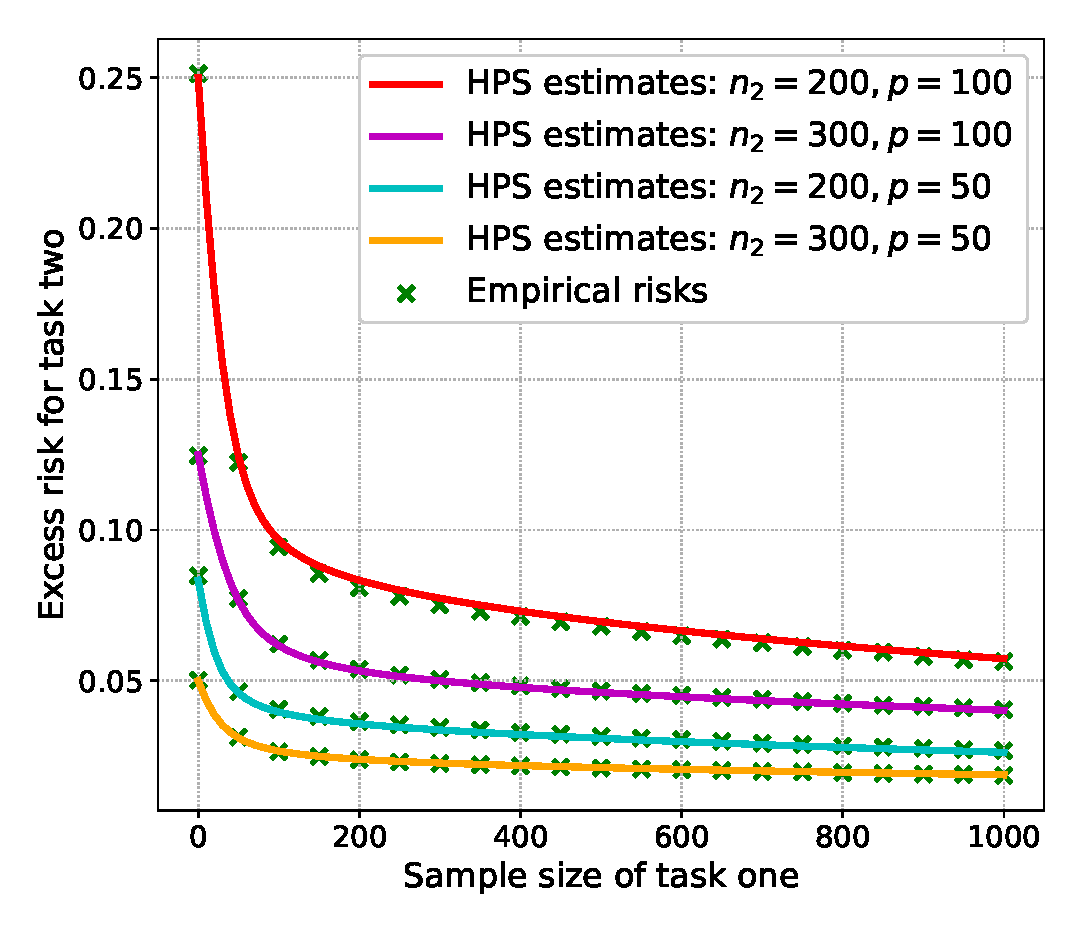
\includegraphics[width=0.9\textwidth]{figures/verify_covariate_shift.eps}
		\caption{Verify variance asymptotics in finite dimensions}
		\label{fig_sec3_verify_cov}
	\end{subfigure}
	\begin{subfigure}[b]{0.5\textwidth}
		\centering
		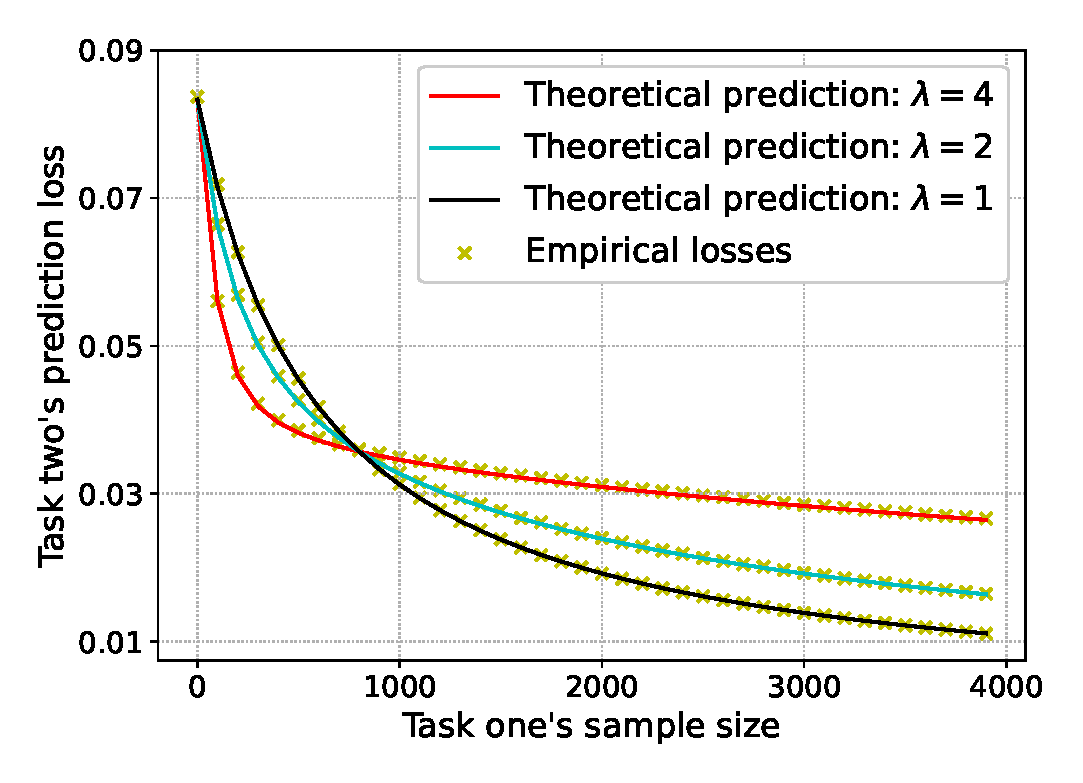
\includegraphics[width=0.9\textwidth]{figures/covariate_shift.eps}
		\caption{Sample size ratios vs. covariate shift}
		\label{fig_sec3_covariate}
	\end{subfigure}
	\caption{Figure \ref{fig_sec3_covariate}: we verify that Theorem \ref{thm_main_RMT} provides incredibly accurate estimates of the empirical variance under various finite sample sizes and dimensions.
	Figure \ref{fig_sec3_covariate}: We illustrate an intriguing dichotomy between covariate shift and sample size ratio: The dimension $p = 200$, $n_2 = 800$, and the noise variance $\sigma^2 = 1/4$.}
	\label{fig_sec31}
\end{figure}

\paragraph{Illustrative examples.}
Next, we illustrate the result of Corollary \ref{cor_hps_cov} in several examples.

\begin{example}[Does covariate shift help or hurt information transfer?]
    Our first example illustrates that the effect of covariate shift depends on the sample sizes of each dataset in an intricate manner.
    While the folklore belief is that transferring from a covariate-shifted distribution performs worse than an identical distribution, we show that, surprisingly, the former can sometimes outperform the latter.
    
    We first describe a setting for modeling covariate shift.
    Let $\cS$ be the set of positive definite matrices $M^{\top} M$ such that for $i = 1,2,\dots,\floor{\frac p 2}$, $\lambda_{p - i}  = \frac 1 {\lambda_i}$, where $\lambda_1 \ge \lambda_2 \ge \cdots \ge \lambda_p$ are the eigenvalues of $M$.
    Under this setting, we ask: suppose that the sample sizes $n_1$ and $n_2$ are both fixed, which $M$ provides the best ``transfer'' in the sense of HPS estimator's excess risk?
    We observe a dichotomy that depends on whether or not $n_1$ is greater than $n_2$.
    \begin{claim}[Covariate shift vs. sample size ratios]\label{claim_dichotomy}
        Let $g(M) = \frac{\sigma^2}{n_1 + n_2} \bigtr{\frac 1 {\alpha_1 M^{\top} M + \alpha_2}}$.
        Suppose that $n_1$ and $n_2$ are both fixed.
        Within the set of all possible covariate shift matrix $M\in\cS$, the following dichotomy holds:
        \begin{itemize}
	        \item If $n_1 \ge n_2$, then $g(M)$ is minimized in $\cS$ when $\lambda_i = 1$, for any $i = 1,\dots,p$.
	        \item If $n_1 < n_2$, then $g(M)$ is maximized in $\cS$ when $\lambda_i = 1$, for any $i = 1,\dots,p$.
        \end{itemize}
    \end{claim}

\begin{proof}
    We explain why the above dichotomy happens. We can write $g(M)$ for any $M \in \cS$ as
    $$g(M)=\frac{\sigma^2}{ n_1+n_2 }\sum_{i=1}^{p/2}\left( \frac{1}{\lambda_i^{2} a_1 + a_2} + \frac1{\lambda_i^{-2} a_1 + a_2} \right).$$
    When $M=\id_{p\times p}$, by the first equation of \eqref{eq_a12extra}, we have
    $$g(\id_{p\times p})=\frac{\sigma^2}{ n_1+n_2 }\sum_{i=1}^{p/2} \frac{2}{1-\gamma},$$
    where we abbreviate $\gamma:=p/(n_1+n_2)$. Then using $\alpha_1 + \alpha_2 = 1-\gamma$, through a direct calculation we find that
    \begin{align*}
        g(M) - g(\id_{p\times p})%&= \frac{\sigma^2 \gamma}{2(1-\gamma)} (\lambda^2-1)a_1\cdot \bigbrace{  \frac{1}{ -a_1(\lambda^2-1)+(1-\gamma)\lambda^2 } - \frac{1}{a_1(\lambda^2-1) + (1-\gamma)}} \\
        &= \frac{\sigma^2 }{ n_1+n_2-p} \sum_{i=1}^{p/2} \frac{(\lambda_i^2-1)^2 \alpha_1 \left[ \alpha_1 - \alpha_2\right] }{[\alpha_1 + \lambda_i^2 \alpha_2][\lambda_i^2 \alpha_1 + \alpha_2]} .
    \end{align*}
    %in this example is equal to
    %$\frac{p}{2(n_1 + n_2)} f(\lambda)$, where
    %\[ f(\lambda) = {(\lambda^{-2} a_1 + a_2)^{-1} + (\lambda^2 a_1 + a_2)^{-1}}. \]
    %Using the fact that $a_1 + a_2 = 1 - \frac{p}{n_1 + n_2}$, we can verify
    %\begin{align*}
    %	f(\lambda) - f(1) &= \left(\lambda^2 a_1 + \frac{n_1 + n_2 - p}{n_1 + n_2} - a_1\right)^{-1} \\
    %	&+ \left(\lambda^{-2} a_1 + \frac{n_1 + n_2 - p}{n_1 + n_2} - a_1\right)^{-1} \\
    %	&- \frac{2(n_1 + n_2)}{n_1 + n_2 - p} \\
    %	&= \left(2a_1 - \frac{n_1 + n_2-p} {n_1 + n_2 }\right)  g(\lambda, a_1), %\cdot (\lambda^2-1)^2
    %\end{align*}
    %\begin{align*}
    %	f(\lambda) - f(1) &= \left(2a_1 - \frac{n_1 + n_2-p} {n_1 + n_2 }\right)  g(\lambda, a_1), %\cdot (\lambda^2-1)^2
    %\end{align*}
    %where $g(\lambda, a_1) \ge 0$.
    %and can be derived from algebraic calculations (details omitted).
    We claim that $\alpha_1 > \alpha_2$ if and only if $n_1 > n_2$, which then explains the dichotomy.
    In fact, if $\alpha_1 > \alpha_2$, then the first part of equation \eqref{eq_a12extra} gives that $\alpha_1 > (1-\gamma)/2$.
    The second part of equation \eqref{eq_a12extra} gives that
    \begin{align*}
     \frac{n_1}{n_1 + n_2} &> \alpha_1 + \frac{1}{n_1+n_2} \sum_{i=1}^{p/2}\left(\frac{\lambda_i^2}{\lambda_i^2+1}+\frac{\lambda_i^{-2}}{\lambda_i^{-2}+1}\right) = \frac{1-\gamma}{2}+\frac{\gamma}{2}=\frac{1}{2}.
    \end{align*}
    %\begin{align*}
    % \frac{n_1}{n_1 + n_2} &=a_1 + \frac1{n_1 + n_2}\cdot \bigbrace{\sum_{i=1}^p \frac{\lambda_i^2 a_1}{\lambda_i^2 a_1 + a_2}} \\
    %	&> a_1 + \frac{p}{2(n_1+n_2)} \left(\frac{\lambda^2}{\lambda^2+1}+\frac{\lambda^{-2}}{\lambda^{-2}+1}\right) =\frac{1}{2}.
    %\end{align*}
    This is equivalent to $n_1>n_2$. The other direction follows from a similar argument. % Similarly, if $a_1<a_2$, equations  \eqref{eq_a12extra000} and  \eqref{eq_a12extra} give that $a_1 < \frac{n_1 + n_2-p}{2 (n_1 + n_2)}$ and $n_1<n_2$. Thus, we conclude that $f(\lambda) \ge f(1)$ if and only if $n_1 \ge n_2$.
    %\end{example}
\end{proof}

Figure \ref{fig_sec3_covariate} illustrates a special case where $\lambda_1 = \cdots = \lambda_{\floor{p /2}} = \lambda > 0$ for $M^{\top}M$ and the rest of the eigenvalues are all equal to $1 / \lambda$.
Thus, $\lambda > 0$ captures the degree of covariate shift: higher $\lambda$ implies worse covariate shift.
We observe that our theoretical estimates using Corollary \ref{cor_hps_cov} matches the empirical risks incredibly accurately.
As a result, we indeed observe the dichotomy shown in Claim \ref{claim_dichotomy}.
Furthermore, for higher $\lambda$, HPS' excess risk decreases slower--indicating a worse rate of ``transfer'' from task one. 
As a remark, the classical work of \citet{david2010impossibility} have likewise shown impossibility results for transfer learning under covariate shift in a classification setting.
By contrast, our analysis applies to a (high-dimensional) regression setting.
\end{example}


\begin{example}
Our second example illustrates that the effect of covariate shift worsens as the sample size of task one increases.
We consider a set of covariate shift matrices $M^{\top} M$ whose determinant are all equal to one, and the eigenvalues are bounded between $\tau^2$ and $1 / \tau^2$.
Let $\cS$ denote the set of $M\in\real^{p\times p}$ such that $M^{\top} M$ satisfies both conditions.
\begin{claim}[Identical covariance provides approximately optimal transfer under imbalanced dataset sizes]\label{prop_covariate}
    Recall that $g(M) = \frac{\sigma^2}{n_1 + n_2} \bigtr{\frac 1 {\alpha_1 M^{\top} M + \alpha_2}}$.
	We have the following result regarding $g(\id_{p \times p})$:
	\begin{align} g(\id_{p\times p}) \le \bigbrace{1+ {\frac{n_2}{\tau^2 n_1}  }} g(M), \text{ for any } M \in \cS. \label{eq_claim_id}
	\end{align}
\end{claim}
\begin{proof}
    We can write down the trace of $(\alpha_1 M^{\top} M + \alpha_2)^{-1}$ using the eigenvalues of $M^{\top} M$ as follows:
    \begin{align*}
        (\alpha_1 M^{\top} M + \alpha_2)^{-1} &= \sum_{i=1}^p \frac{1} {\alpha_1 \lambda_i^2 + \alpha_2} \\
        &\ge \sum_{i=1}^p \frac{1} {\alpha_1 \lambda_i^2 + \alpha_2 \cdot {\lambda_i^2} / {\tau^2}} \tag{since $\lambda_i \ge \tau$, for any $i$} \\
        &= \frac 1 {\alpha_1 + \alpha_2 / \tau^2} \sum_{i=1}^ p \frac 1 {\lambda_i^2} \\
        &\ge \frac 1 {\alpha_1 + \alpha_2 /\tau^2} p\cdot \bigbrace{\prod_{i=1}^p \frac 1 {\lambda_i^2}}^{1/ p} \tag{by the AM-GM inequality} \\
        &= \frac{p}{\alpha_1 + \alpha_2 / \tau^2} \tag{since $\prod_{i=1}^p \lambda_i^2 = \det(M^{\top} M) = 1$}
    \end{align*}
    Next, recall from equation \eqref{g_id} that
    $g(\id_{p\times p}) = \frac{\sigma^2 p}{n_1 + n_2 - p}$.
    Thus, equation \eqref{eq_claim_id} follows if we show that (after rearranging terms)
    \begin{align}
        \frac{n_1 + n_2}{n_1 + n_2 - p} \cdot \frac 1 {\alpha_1 + \frac{\alpha_2}{\tau^2}} \le 1 + \frac{n_2}{\tau^2 \cdot n_1}. \label{eq_claim_id_step}
    \end{align}
    From the second part of equation \eqref{eq_a12extra}, we have that
    \begin{align*}
        \frac{n_1} {n_1 + n_2} &= \alpha_1 + \frac 1 {n_1 + n_2} \bigbrace{\sum_{i=1}^p \frac{\lambda_i^2\alpha_1}{\lambda_i^2\alpha_1 + \alpha_2}} \\
        &< \alpha_1 + \frac p {n_1 + n_2}.
    \end{align*}
    Thus, $\alpha_1 > \frac{n_1 - p}{n_1 + n_2}$, which implies that $\alpha_2 < \frac{n_2}{n_1 + n_2}$.
    Hence, $\alpha_1 + \frac{\alpha_2}{\tau^2} = 1 - \frac{p}{n_1 + n_2} - \alpha_2 + \frac{\alpha_2}{\tau^2} \le 1 - \frac{p}{n_1 + n_2} + \frac{n_2}{n_1 + n_2} \frac 1 {\tau^2}$, which implies
    equation \eqref{eq_claim_id_step} by straightforward calculations.
    Thus, the proof is complete.
\end{proof}
As a corollary of Claim \ref{prop_covariate}, when $n_1$ is much larger than $n_2 / \tau^2$, the excess risk of HPS is approximately optimal in the set of all possible $M\in\cS$ when there is no covariate shift between dataset one and two.
\end{example}





\subsection{Model shift}\label{sec_sizeratio}

 In this subsection, we consider the setting where $X^{(1)}$ and $X^{(2)}$ are independent and have the same population covariance matrices $\Sigma^{(1)}=\Sigma^{(2)}$. However, the two tasks can have different sample sizes $n_1\ne n_2$. In this case, we can obtain the exact asymptotic limits of the bias term \eqref{Lbias} and the variance term \eqref{Lvar}. We will use these results to illustrate the effects of the bias-variance tradeoff and varying sample sizes on the performance of the $\MTL$ estimator.

\begin{theorem}[Excess risk of HPS under model shift]\label{cor_MTL_loss}
Under Assumption \ref{assm_big1}, suppose that $\Sigma^{(1)}=\Sigma^{(2)}$ and the entries of $Z^{(1)}$ and $Z^{(2)}$ are i.i.d. Gaussian random variables. Then for any small constant $\e>0$ and large constant $C>0$, there exists a high probability event $\Xi$, on which the following estimates hold uniformly in all $a\in \R$:
\be\label{Lvar_samplesize}
L_{\var}(a)= \sigma^2  \left[ \cal L_1(a)+ \OO\left({p^{c}}/{n_1}\right)\right]  ,
\ee
and
\begin{align}
L_{\bias}(a)&= \left[ \cal L_2(a)+  \OO\left(p^{-1/2+c}\right)\right] \cdot  \|\beta^{(1)}-a\beta^{(2)}\|^2 \nonumber\\
&+ \OO \left[ p^{-C}\left( \|\beta^{(1)} \|^2  +  \|\beta^{(2)} \|^2\right)   \right].\label{Lbias_samplesize}
	%-\left[1- \left( 1-\frac{1}{\sqrt{\rho_1}}\right)^4\right] pd^2\cdot \frac{\rho_1^2 (\rho_1+\rho_2)}{(\rho_1 + \rho_2 - 1)^3} +\OO(p^{-c}\sigma^2)  \le
	%   \left|L(\hat{\beta}_2^{\MTL}) - \frac{2d^2 n_1^2 (n_1 + n_2)}{(n_1 + n_2 - p)^3} -\frac{\sigma^2 p}{n_1 + n_2 - p}  \right|
	% \le \varepsilon \cdot \frac{2d^2 n_1^2 (n_1 + n_2)}{(n_1 + n_2 - p)^3} +  \OO(p^{-c/2}).\label{cor_MTL_error}
	%\left[\left( 1+\frac{1}{\sqrt{\rho_1}}\right)^4-1\right] d^2\cdot \frac{\rho_1^2 (\rho_1+\rho_2)}{(\rho_1 + \rho_2 - 1)^3} \\
	%& +C \left[(p^{-c_\varphi}+p^{-c_\infty/2})(\sigma^2 +d^2)+p^{-c_\infty}\kappa^2 + %\frac{d^4+\sigma^2 d^2}{\kappa^2}\right],\nonumber
	 \end{align}
Here we define the functions
\begin{align*}
&\cal L_1(a):= \frac{2p}{  {n_2} (1-\xi_2) + a^2 n_1 (1-\xi_1)+ \sqrt{[ {n_2} (1-\xi_2) +a^2 n_1 (1-\xi_1)]^2 + 4a^2{n_2}{n_1} (\xi_1+\xi_2 -\xi_1\xi_2)}}, \\
&\cal L_2(a): = \frac1{a^2}\cdot \frac{1- 2\frac{\cal L_1(a)}{\xi_2[1 + \cal L_1(a)]} + \kappa(a)}{1- \xi_2 \kappa(a)},
\end{align*}
where we abbreviate $\xi_1:=p/n_1$, $\xi_2:=p/n_2$ and
\begin{align*}
\kappa(a):= \frac{\cal L_1(a)^2}{\xi_2^2[1+\cal L_1(a)]^2}  \left[1 - \frac{a^4 \cal L_1(a)^2 }{\xi_1[1+a^2\cal L_1(a) ]^2}\right]^{-1}.
%f_2(a):= \frac{a^4 \cal L_1(a)^2}{\xi_1^2 } \left[1 - \frac{a^4 \cal L_1(a)^2 }{\xi_1[1+a^2\cal L_1(a) ]^2}\right]^{-1},\\
%f_3(a):= \frac1{a^2}\frac{\xi_1}{\xi_2 +\cal L_1(a)}
 \end{align*}
%	In the setting of Example \ref{ex_sample_ratio}, assume that
%	%a) the sample sizes $n_1$ and $n_2$ are greater than $(1 + \tau) p$, b) $\Sigma_1=\Sigma_2=\id_p$, and c) %there exists a small constant $c_0>0$ such that
%	(i) both tasks sample sizes are at least $3p$;
%	(ii) noise variance is smaller than the shared signal variance: $\sigma^2 \lesssim  \kappa^2$;
%%	\be\label{choiceofpara0}
%%	p^{-1/2+c_0}\sigma^2 + p^{c_0}d^2\le \kappa^2\le p^{1-c_0} (\sigma^2 +d^2)  .  	\ee
%	%\be\label{choiceofpara0}
%%	(ii) the task-specific variance of $\beta_i$ is much smaller than the signal strength {\color{red}$d^2 = \oo( {\kappa^2})$}; \HZ{what does $\ll$ mean exactly?}
%%	(iii) the sample sizes $n_1$ and $n_2$ are greater than $(1 + \tau) p$.
%	(iii) task-specific variance is much smaller than the shared signal variance: $d^2 \le p^{-\e}{\kappa^2}$ for a small constant $c>0$.
%	Let $\varepsilon = (1 + \sqrt{p/n_1})^ 4 - 1$, which decreases as $n_1$ increases.
%	Let $\hat{A},\hat{B}$ be the global minimizer of $f(A, B)$.
%	With high probability over the randomness of the input,
%	the prediction loss of $\hat{\beta}_2^{\MTL} = \hat{B} \hat{A}_2$ for task two satisfies that
%	\begin{align}
%	%-\left[1- \left( 1-\frac{1}{\sqrt{\rho_1}}\right)^4\right] pd^2\cdot \frac{\rho_1^2 (\rho_1+\rho_2)}{(\rho_1 + \rho_2 - 1)^3} +\OO(p^{-c}\sigma^2)  \le
%	   \left|L(\hat{\beta}_2^{\MTL}) - \frac{2d^2 n_1^2 (n_1 + n_2)}{(n_1 + n_2 - p)^3} -\frac{\sigma^2 p}{n_1 + n_2 - p}  \right|
%	\le \varepsilon \cdot \frac{2d^2 n_1^2 (n_1 + n_2)}{(n_1 + n_2 - p)^3} +  \OO(p^{-c/2}).\label{cor_MTL_error}
%	%\left[\left( 1+\frac{1}{\sqrt{\rho_1}}\right)^4-1\right] d^2\cdot \frac{\rho_1^2 (\rho_1+\rho_2)}{(\rho_1 + \rho_2 - 1)^3} \\
%	%& +C \left[(p^{-c_\varphi}+p^{-c_\infty/2})(\sigma^2 +d^2)+p^{-c_\infty}\kappa^2 + %\frac{d^4+\sigma^2 d^2}{\kappa^2}\right],\nonumber
%	 \end{align}
%	 with high probability for any fixed $c\in(0, \min(\frac{1}{4}, \delta,\frac{\varphi-4}{2\varphi}))$.
%	 {\color{red}[FY: the error also contains $p^{-1/2+2c}\kappa^2 +  p^{-1/4+c} (\sigma^2 +d^2) $, both of which cannot be omitted, because (i) there is no assumption on the upper bound of $\kappa^2$, and (ii) we do not necessarily have $c_\varphi<1/4$. We can decide how to present the result concisely (for instance we can impose an upper bound on $\kappa^2$ and that $c_\varphi<1/4$), but it needs to be correct.]}
	 \end{theorem}

\iffalse
 We need to state a result for Gaussian matrix ...... Consider
$$f (\al,n_1,n_2)= \frac1p\tr\left[\frac{1}{ (X_1^\top X_1 + \al \cdot X_2^\top X_2)^2} (X_1^\top X_1)^2\right].$$
In our case, we have $\al=1$, but we can handle more general $\al$. We introduce two parameters:
$$a= \al \frac{n_2}{n_1} \left( \frac{p}{n_1} + \frac{p}{n_2}- \frac{p}{n_1 }\cdot \frac{p}{n_2}\right),\quad b= \al \frac{n_2}{n_1}\left( 1- \frac{p}{n_2}\right) + \left( 1- \frac{p}{n_1}\right). $$
Then we define the following parameters:
\begin{align*}
x= \frac{-b+ \sqrt{b^2 + 4a}}{2a},\quad y= \left[ x^{-2} - \frac{p}{n_1}\left( 1+\frac{p}{n_1}x\right)^{-2}\right]^{-1},\quad \omega= \al\frac{n_2}{n_1} \left( 1 + \al \frac{p}{n_1}x\right)^{-1}.
\end{align*}
We have that
$$f(\al,n_1,n_2)= \frac{1 - 2\omega x + \omega^2 y}{ 1 - \frac{p}{n_2} \cdot \omega^2 y } +\oo(1)\quad \text{w.h.p.} $$
In the setting $\al=1$, both $\omega x$ and $\omega^2 y$ can be written in terms of only one parameter
%$$f(\al,n_1,n_2)= \frac{\left(u^2 -\frac{p}{n_1}\right) \left(1- 2\frac{n_2}{n_1}  u^{-1}\right) + \frac{n_2^2}{n_1^2} }{ u^2 -\frac{p}{n_1}\left(1 + \frac{n_2}{n_1}\right) } +\oo(1)\quad \text{w.h.p.} $$
%where
$$u: = x^{-1}\left(1+\frac{p}{n_1}x\right)=   \frac{ b+\sqrt{b^2+4a}}{2} +\frac{p}{n_1}   .$$
\fi

We believe the convergence rates $p^c/n_1$ and $p^{-1/2+c}$ in \eqref{Lvar_samplesize} and \eqref{Lbias_samplesize} are both sharp up to the $p^c$ factor. The proof of Theorem \ref{cor_MTL_loss} will be given in Appendix \ref{app_iso_cov} in the supplement \cite{MTL_suppl}. For the variance estimate in \eqref{Lvar_samplesize}, it is not necessary to assume the Gaussian distributions of the $Z^{(1)}$ and $Z^{(2)}$ entries. In fact, \eqref{Lvar_samplesize} is a special case of Theorem \ref{thm_main_RMT} below for the more general case with possibly different $\Sigma^{(1)}$ and $\Sigma^{(2)}$. On the other hand, the Gaussian assumption is needed in our current proof of the bias limit \eqref{Lbias_samplesize}. In the setting of Theorem \ref{cor_MTL_loss}, we can write
\begin{align*}
L_{\bias} (a)&=\bv_a^\top (Z^{(1)})^\top Z^{(1)} \frac1{ \left[a^2(Z^{(1)})^\top Z^{(1)}+ (Z^{(2)})^\top Z^{(2)}  \right]^{2}}(Z^{(1)})^\top Z^{(1)} \bv_a,
\end{align*}
where we abbreviate $\bv(a):=(\Sigma^{(1)})^{1/2}\left(a\beta^{(1)}- a^2\beta^{(2)}\right)$. By the rotational invariance of $(Z^{(1)})^\top Z^{(1)}$ and $(Z^{(2)})^\top Z^{(2)}$, we have that
\begin{align}\label{Lbias_idea}
L_{\bias} (a)&\approx \|\bv_a\|^2 \frac1p\bigtr{ [(Z^{(1)})^\top Z^{(1)}]^2 \frac1{ \left[a^2(Z^{(1)})^\top Z^{(1)}+ (Z^{(2)})^\top Z^{(2)}\right]^{2}}  },
\end{align}
up to a small error. Notice that we can write \eqref{Lbias_idea} into a simpler form
\begin{align}\nonumber %\label{Lbias_idea2}
L_{\bias} (a)&\approx \|\bv_a\|^2 \left. \frac{\dd }{\dd x}\right|_{x=0}\frac1p\bigtr{  \frac1{ a^2(Z^{(1)})^\top Z^{(1)}+ x[(Z^{(1)})^\top Z^{(1)}]^2+(Z^{(2)})^\top Z^{(2)} }  }.
\end{align}
It is well-known that the empirical spectral distributions (ESD) of $(Z^{(i)})^\top Z^{(i)}$, $i=1,2$, satisfy the famous Marchenko-Pastur (MP) law asymptotically \cite{MP}. From the MP law of $(Z^{(1)})^\top Z^{(1)}$, we can also derive the asymptotic ESD of $a^2(Z^{(1)})^\top Z^{(1)}+ x[(Z^{(1)})^\top Z^{(1)}]^2$ for any fixed $a\in \R$ and $x>0$. Due to the rotational invariance of multivariate Gaussian distributions,
%$a^2(Z^{(1)})^\top Z^{(1)}+ x[(Z^{(1)})^\top Z^{(1)}]^2$ and $(Z^{(2)})^\top Z^{(2)}$ are asymptotically freely independent from each other \cite{nica2006lectures}. Hence
the asymptotic ESD of $a^2(Z^{(1)})^\top Z^{(1)}+ x[(Z^{(1)})^\top Z^{(1)}]^2+(Z^{(2)})^\top Z^{(2)}$ is given by the free additive convolution (or free addition) of the asymptotic ESD of $a^2(Z^{(1)})^\top Z^{(1)}+ x[(Z^{(1)})^\top Z^{(1)}]^2$ and the MP law of $(Z^{(2)})^\top Z^{(2)}$\cite{nica2006lectures}. In particular, a sharp convergence estimate has been proved in \cite{BES_free1,BES_free2} for the free addition of two probability measures. We use that result to obtain a convergence estimate on
$$\frac1p\bigtr{  \frac1{ a^2(Z^{(1)})^\top Z^{(1)}+ x[(Z^{(1)})^\top Z^{(1)}]^2+(Z^{(2)})^\top Z^{(2)} }  }.$$
Taking derivative with respect to $x$ at $x=0$ gives the exact asymptotic limit of $L_{\bias}(a)$. We refer the reader to Appendix \ref{app_iso_cov} of the supplement \cite{MTL_suppl} for more details.

We believe that the above argument can be extended to the case without the Gaussian assumption. For example, instead of using the results in \cite{BES_free1,BES_free2} on free addition, we can use the sharp local laws on polynomials of random matrices in \cite{EKN_poly}. However, to apply the result in \cite{EKN_poly}, we need to check some difficult technical regularity conditions for our setting, which is not the focus of this work. Hence we do not pursue this direction in this paper.


\paragraph{Illustrative examples.}
Combining Lemma \ref{lem_HPS_loss}, Theorem \ref{cor_MTL_loss} and Proposition \ref{lem_hat_v}, and using  that $\|\beta^{(1)}-\beta^{(2)}\|^2 = (2+\oo(1))d^2$ with high probability, the predication loss $L(\hat{\beta}_2^{\MTL}(\hat a)) $ is approximately equal to
$$\ell(n_1,n_2)= \sigma^2 \cal L_1(1) +   2d^2 \cal L_2(1)= \frac{p\sigma^2}{n_1+n_2-p} +  2d^2  \frac{n_1^2 (n_1+n_2-p)+p n_1n_2}{(n_1+n_2)^2(n_1+n_2-p)}, $$
with high probability, where in the second step we obtain $\cal L_1(1)$ and $\cal L_2(1)$ through direct calculations.
Now we compare $\ell(n_1,n_2)$ with \eqref{L_STL_simple01}. First, we notice that the variance term $\sigma^2 \cal L_1(1)$ is smaller than $L(\hat{\beta}_2^{\STL} )$, while the bias term always increases (because the bias in single-task linear regression is zero). This gives a \emph{bias-variance tradeoff} for the predication loss of the HPS estimator. Second, calculating the derivative with respect to $n_1$, it is not hard to see that the variance term always decreases as $n_1$ increases, while the bias term always increases with $n_1$. Hence how the performance of the HPS estimator changes with respect to $n_1$ also depends on an intricate bias-variance tradeoff.

Now fix an $n_2$, we study the bias-variance tradeoff with respect to $n_1$ using the following function of $\rho:=\rho_1+\rho_2$, which is $L(\hat{\beta}_2^{\STL} )-\ell(n_1,n_2)$ divided by $2d^2$:
$$h(\rho):=\frac{p }{n_2-p}\cdot \frac{\sigma^2}{2d^2}- \frac{\ell(\rho_1p , \rho_2p)}{2d^2}  = \frac{\rho-\rho_2}{(\rho-1)(\rho_2-1)}\cdot \frac{\sigma^2}{2d^2}- \frac{(\rho-\rho_2)^2 (\rho-1)+(\rho-\rho_2)\rho_2}{\rho^2(\rho-1)}  .$$
This function characterizes $L(\hat{\beta}_2^{\STL} )-L(\hat{\beta}_2^{\MTL}(\hat a)) $, and hence gives the quantitive information transfer from the source task to the target task.
First, we have positive (resp. negative) transfer if and only if $h(\rho)>0$ (resp. $h(\rho)<0$). Moreover, the sign of $h(\rho)$ is determined by the sign of the second order polynomial %which is equivalent to the following inequality:
\be\label{poly1} \left( \frac{1}{\rho_2-1}\cdot \frac{\sigma^2}{2d^2}-1 \right)\rho^2 + ( \rho_2+1)\rho - 2\rho_2 .\ee
We observe the following dichotomy. %\FY{add several plots to illustrate this dichotomy}
\begin{enumerate}
\item If $\frac{1}{\rho_2-1}\cdot \frac{\sigma^2}{2d^2}-1 >0$, then the polynomial \eqref{poly1} is positive for all $\rho\in (\rho_2+1,\infty)$, so that the transfer is always positive.

\item If $\frac{1}{\rho_2-1}\cdot \frac{\sigma^2}{2d^2}-1 < 0$, then we have the following cases.

\begin{itemize}
\item If $(\rho_2+1)^2 < 8\rho_2 \left( 1- \frac{1}{\rho_2-1}\cdot \frac{\sigma^2}{2d^2}  \right)$, the polynomial \eqref{poly1} is negative for all $\rho$, so that the transfer is always negative.

\item If $(\rho_2+1)^2 > 8\rho_2 \left( 1- \frac{1}{\rho_2-1}\cdot \frac{\sigma^2}{2d^2}  \right)$, the polynomial \eqref{poly1} has two positive roots, where one of them is always smaller than $\rho_2+1$. Hence if the larger root, say $\rho_c$, is smaller than $\rho_2+1$, then the transfer is always negative for $\rho\in (\rho_2+1,\infty)$; otherwise, there is a transition from positive transfer to negative transfer as $\rho$ crosses $\rho_c$.
\end{itemize}
\end{enumerate}
Second, we calculate the derivative of $h(\rho)$, and find that its sign  is determined by the sign of the third order polynomial
\be\label{poly2}
 \frac{1}{\rho_2}\cdot \frac{\sigma^2}{2d^2} \rho^3 - 2(\rho-\rho_2)(\rho-1)(\rho-2)   - (\rho_2-1)\rho .\ee
Then we observe the following dichotomy. %\FY{add several plots to illustrate this dichotomy}
\begin{enumerate}
\item If $\frac{1}{\rho_2}\cdot \frac{\sigma^2}{2d^2} > 2$, the polynomial \eqref{poly2} is always positive for all $\rho\in (\rho_2+1,\infty)$, so that the information transfer always increases as $n_1$ increases.

\item If $\frac{1}{\rho_2}\cdot \frac{\sigma^2}{2d^2} < 2$, the polynomial \eqref{poly2} is positive initially around $\rho=\rho_2+1$, and then becomes negative when $\rho$ crosses its unique root, say $\rho_c$, in $(\rho_2+1,\infty)$. Hence the information transfer achieves the global maximum at $\rho=\rho_c$.
\end{enumerate}

%where $w_0:={\sigma^2}/{2d^2}$ is the ratio between the model bias and the noise variance.
%and $$ h_1(\rho_1,\rho_2):= \frac{\rho_1}{(\rho_1+\rho_2-1)(\rho_2-1)},\quad h_2(\rho_1,\rho_2):= \frac{\rho_1^2 (\rho_1+\rho_2-1)+\rho_1\rho_2}{(\rho_1+\rho_2)^2(\rho_1+\rho_2-1)}.$$
\iffalse
Then whether $L(\hat{\beta}_2^{\MTL}(\hat a)) $ is larger or smaller than

Applying Theorem \ref{thm_main_RMT} to the above setting, we get that
	\begin{align*}
		\frac{1}{n_1 + n_2} \tr[\Sigma^{(2)} (a_1\Sigma^{(1)} + a_2\Sigma^{(2)})^{-1}]
		= \frac{1}{n_1 + n_2} \bigtr{((a_1 + a_2)\id_p)^{-1}}
		= \frac{p}{n_1 + n_2 - p},
	\end{align*}
	because $a_1 + a_2 = 1 - \frac{p}{n_1 + n_2}$ by equation \eqref{eq_a12extra}.
	%Similarly, for the bias limit, we solve the self-consistent equations \eqref{eq_a34extra} to get $a_3$ and $a_4$ after we have obtained $a_1, a_2$.
	Similarly, we can calculate the bias limit.
	Combined together, we obtain the following corollary of Theorem \ref{thm_main_RMT}.

In the above inequality, the $d^2$ scaling term is the bias limit and the $\sigma^2$ scaling term is the variance limit.
This result allows for a more concrete interpretation since the dependence on datasets' properties is explicit.
The proof of Corollary \ref{cor_MTL_loss} can be found in Appendix \ref{app_iso_cov}.
As a remark, %in equation \eqref{cor_MTL_error}, the predication loss $L(\hat{\beta}_2^{\MTL}) $ was obtained using the global minimizer $(\hat A,\hat B)$. B
by combining the bias and variance limits, we can also obtain a bias-variance tradeoff for any local minimizer of $f(A, B)$.
The proof is similar to Corollary \ref{cor_MTL_loss}, so we omit the details.

{\cor
For the variance term, using equation \eqref{lem_cov_shift_eq}, we obtain that
\be\label{eq_var111}\tr[\hat\Sigma^{-1}] = \tr\left[ \left((X^{(1)})^\top X^{(1)}  + (X^{(2)})^\top X^{(2)}\right)^{-1}\right]=\bigtr{\frac{(a_1 +a_2)^{-1}\id_{p\times p}}{n_{1}+n_2} }+\OO(p^{-c_\varphi})\ee
with high probability. Solving equation \eqref{eq_a12extra} with $\lambda_i\equiv 1$, $1\le i\le p$, we get that
	\begin{align}
		 a_1 = \frac{n_1(n_1 + n_2 - p)}{(n_1 + n_2)^2} ,\quad
		& a_2 = \frac{n_2(n_1 + n_2 - p)}{(n_1 +n_2)^2} . \label{simplesovlea12}
			\end{align}
Applying the above to equation \eqref{eq_var111}, we obtain that with high probability
\be\label{eq_var112}\tr[\hat\Sigma^{-1}]  = \frac{p}{n_1+n_2} \cdot \frac{n_1+n_2}{n_1+n_2-p}+\OO(p^{-c_\varphi})=  \frac{p}{n_1+n_2-p}+\OO(p^{-c_\varphi}).\ee
For the bias term,
}


Next, we use the bias-variance limits to study how varying sample sizes impacts HPS.
For example, imagine if we want to decide whether to collect more of task one's data or not, how does increasing $n_1$ affect the prediction loss?
We assume that $n_2$ is fixed for simplicity.
%Now we illustrate an interesting phenomenon that adding task one's samples helps task two initially, but may hurt eventually.
The variance limit in equation \eqref{cor_MTL_error} obvious decreases with $n_1$.
It turns out that the bias term always increases with $n_1$, which can be verified by showing that the bias limit's derivative is always nonnegative.
%As a function of the sample ratio, the limiting estimate always decreases first from $\frac{\sigma^2 p}{n_2 - p}$ with $n_1$ being zero, and then increases to $d^2$ when $n_1$ goes to infinity.
%We describe a sketch of the proof.
By comparing the derivative of the bias and variance limits with respect to $n_1$ (details omitted), we obtain the following dichotomy.
\begin{enumerate}
	\item When $\frac{d^2}{\sigma^2} < \frac{p}{4n_2 - 6p}$, the prediction loss decreases monotonically as $n_1$ increases.
	Intuitively, this regime of $d^2$ always helps task two.
	\item When $\frac{d^2}{\sigma^2} > \frac{p}{4n_2 - 6p}$, the prediction loss always decreases first from $\frac{\sigma^2 p}{n_2 - p}$ (when $n_1 = 0$), and then increases to $d^2$ (when $n_1 \rightarrow \infty$).
	To see this, near the point where $n_1$ is zero, one can verify (from the derivatives) that bias increases less while variance decreases more, and there is \textit{exactly} one critical point where the derivative is zero, which corresponds to the \textit{optimal sample size ratio}.
\end{enumerate}
\fi
%	\end{example}

%\paragraph{Comparing HPS to other estimators.}

\todo{merge into prev paragraphs {Simulations.}}
Second, we validate the result of Example \ref{ex_sample_ratio}.
Figure \ref{fig_size} shows task two's prediction loss  as we increase the sample ratio $n_1 / n_2$ from $1/10$ to $7/10$.
%Again, our estimates are accurate compared to the empirical losses.
We consider a regime where task two consists of $80,000$ samples, and task one's sample size varies from $8,000$ to $56,000$.
The task-specific variance (which scales with model distance) is $d = 0.2$, the noise variance is $\sigma^2 = 4^2$, and the shared signal variance is $1$. We observe that as we increase the sample ratio, task two's prediction loss decreases initially but later will increase when the sample ratio is above a certain level.
On the other hand, when $d = 0.15$, task two's prediction loss decreases faster.
Intuitively, this is because bias increases less for smaller $d^2$.





\subsection{Covariate and model shift}


For the bias limit, we have the following proposition.

\begin{theorem}[Bias estimates under covariate and model shift]\label{prop_main_RMT}
%The bias equation \eqref{Lbias} satisfies the following limit with high probability: Let $S$ be an arbitrary subset of the unit sphere in dimension $p$ whose size is polynomial in $p$, for any unit vector $w\in S$,
Under Assumption \ref{assm_big1}, for any small constant $c>0$ and large constant $C>0$, there exists a high probability event $\Xi$, on which the following estimate  holds for $L_{\bias}(a)$ in \eqref{Lbias}:
			\begin{align}
				& \bigabs{ L_{\bias}(a) -   (\beta^{(1)}- a\beta^{(2)} )^\top (\Sigma^{(1)})^{1/2} \Pi(a)(\Sigma^{(1)})^{1/2} (\beta^{(1)}- a\beta^{(2)})   }  \nonumber\\
				& \le \left[\left( 1+\sqrt{\frac{p}{n_1}}\right)^4 - 1 +\OO\left( n_1^{-1/2+2/\varphi + c}\right)\right] \frac{n_1^2 \lambda_1^2 \left\|(\Sigma^{(1)})^{1/2} \left(\beta^{(1)}- a\beta^{(2)}\right) \right\|^2}{  [(\sqrt{n_1}-\sqrt{p})^2 \lambda_p^2+ (\sqrt{n_2}-\sqrt{p})^2]^2}  \nonumber\\
				& + p^{-C} \left[\| \beta^{(1)}\|^2 + \| \beta^{(2)}\|^2 \right], \label{lem_cov_derv_eq}
			\end{align}
%			\begin{align}\label{lem_cov_derv_eq}
%				\bigabs{ L_{\bias}(a) - \left\|\frac{n_1}{n_1+n_2}  \frac{\left[a_3 M(a)^\top M(a) + (a_4 + 1) \right]^{1/2}}{ a_1 M(a)^\top M(a) + a_2 } M(a)^\top (\Sigma^{(1)})^{1/2} \left(\beta^{(1)}- a\beta^{(2)}\right)\right\|^2   } \le  \frac{p^{-c_{\varphi}}}{(n_1+n_2)^2},
%			\end{align}
				uniformly in all $a\in \R$. Here $\lambda_1$ and $\lambda_p$ are respectively the largest and smallest singular values of $M(a)$, $\Pi(a)$ is a $p\times p$ matrix defined as
				$$\Pi(a):=\frac{n_1^2}{(n_1+n_2)^2}  M(a)  \frac{a_3 M(a)^\top M(a) + (a_4 + 1) }{[a_1 M(a)^\top M(a) + a_2 ]^2} M(a)^\top  ,$$
				 and $(a_{3},a_4)$ is the solution of the following system of equations % with $b_k = \frac1{p}\sum_{i=1}^p \frac{\lambda_i^{2k}} {(\lambda_i^2 a_1 + a_2)^2}$, for $k = 0, 1, 2$:
		\be  \label{eq_a34extra}
		\begin{split}
				& a_3 + a_4 = \frac{1}{n_1 + n_2}\sum_{i=1}^p \frac{1}{\lambda_i^2 a_1 + a_2}, \\
				& a_3 + \frac{1}{n_1 + n_2} \sum_{i=1}^p \frac{\lambda_i^2 (a_2 a_3-a_1 a_4 )}{(\lambda_i^2 a_1 + a_2)^2} = \frac{1}{n_1 + n_2} \sum_{i=1}^p \frac{\lambda_i^2 a_1}{(\lambda_i^2 a_1 + a_2)^{2}},
%				\left(\frac{\rho_1}{a_1^{2}} -  b_2  \right)\cdot  a_3 -  b_1 \cdot  a_4 = b_1,\quad \left(\frac{\rho_2}{a_2^{2}}-  b_0\right)\cdot  a_4 - b_1 \cdot  a_3
%				= b_0.
			\end{split}
			\ee
			where we recall that $(a_1,a_2)$ is the solution of \eqref{eq_a12extra}.
\end{theorem}

Note that the first error term on the right-hand side of \eqref{lem_cov_derv_eq} is typically smaller than the main term $ (\beta^{(1)}- a\beta^{(2)} )^\top (\Sigma^{(1)})^{1/2} \Pi(a)(\Sigma^{(1)})^{1/2} (\beta^{(1)}- a\beta^{(2)})  $ by a factor of $\OO(\sqrt{p/n_1} + n_1^{-1/2+2/\varphi + c})$. Hence \eqref{lem_cov_derv_eq} only gives an exact asymptotic limit in the regime $n_1\gg p$. Moreover, by equations \eqref{eq_a12extra} and \eqref{eq_a34extra} we have
$$a_1 =\frac{n_1}{n_1+n_2} + \OO\left( \frac{p}{n_1+n_2}\right), \quad a_3 =\frac{n_3}{n_1+n_2} + \OO\left( \frac{p}{n_1+n_2}\right),$$
and
$$a_3 =\OO\left( \frac{p}{n_1+n_2}\right),\quad a_4 =\OO\left( \frac{p}{n_1+n_2}\right).$$
Using these estimates, it is easy to check that
\begin{align}
& (\beta^{(1)}- a\beta^{(2)} )^\top (\Sigma^{(1)})^{1/2} \Pi(a)(\Sigma^{(1)})^{1/2} (\beta^{(1)}- a\beta^{(2)})   \nonumber \\
&=\left\| (\Sigma^{(2)})^{1/2}\frac{1}{a^2\Sigma^{(1)}+\Sigma^{(2)}} a \Sigma^{(1)} \left(\beta^{(1)}- a\beta^{(2)}\right) \right\|^2 + \OO\left( \frac{p\left\|\beta^{(1)}- a\beta^{(2)}\right\|^2}{n_1+n_2}  \right)  . \label{bias_LLN}
\end{align}
Hence \eqref{lem_cov_derv_eq} is consistent with the result obtained by replacing $ (X^{(1)})^\top X^{(1)}$ and $ (X^{(2)})^\top X^{(2)}$ with $n_1\Sigma^{(1)}$ and $n_2\Sigma^{(2)}$, respectively, in $L_{\bias} (a) $ using the law of large numbers in the regime $n_1\gg p$. However, simulations show that our estimate \eqref{lem_cov_derv_eq} is more precise than the first term on the right-hand side of \eqref{bias_LLN}.

\begin{remark}
%First, our result in Corollary \ref{cor_MTL_loss} involves an error term that scales down with $n_1$.
%Tightening this error bound requires showing the limit of $\normFro{({Z^{(1)}}^{\top} Z^{(1)} + {Z^{(2)}}^{\top} Z^{(2)})^{-1} {Z^{(1)}}^{\top} Z^{(1)}}^2$ for two isotropic sample covariance matrices.
%This requires studying the asymptotic singular values distribution of the non-symmetric matrix $({Z^{(1)}}^{\top} Z^{(1)})^{-1}{Z^{(2)}}^{\top} Z^{(2)}+\id$, which is still an open problem in random matrix theory.
%\begin{remark}
The main error in Proposition \ref{prop_main_RMT} comes from approximating $(Z^{(1)})^\top Z^{(1)}$ by $n_1\id_{n_1\times n_2}$ using Corollary \ref{fact_minv} in the supplement \cite{MTL_suppl}. In order to improve this estimate and obtain an exact asymptotic result, one needs to study the singular value distribution of the  random matrix $\cal X + a^2$ for any fixed $a\in \R$, where $\cal X:=[(X^{(1)})^{\top}X^{(1)}]^{-1}(X^{(2)})^{\top}X^{(2)}$. We remark that the eigenvalues of $\cal X$ have been studied in the name of Fisher matrices \cite{Fmatrix}. However, since $\cal X$ is not symmetric, its singular values are different from its eigenvalues. To the best of our knowledge, the asymptotic singular value behavior of $\cal X$ is still an open problem in random matrix theory, and the study of the singular values of $\cal X + a^2$ will be even harder. We leave this problem to future study.

We also remark for the general case with covariate shift, the method in Section \ref{sec_sizeratio} for the bias term also fails, because we cannot reduce the problem into the free addition of two random matrices that are asymptotically freely independent.
%\end{remark}
\end{remark}

\todo{describe comparison to the TL estimator and the weighted OLS estimator.}
	\section{Empirical results}\label{sec_exp}

This section complements our theoretical analysis of HPS with empirical evaluations.
First, we evaluate the performance of HPS estimators against several natural transfer learning estimators.
We show that HPS achieves superior performance under various settings of covariate and model shifts.
Second, we provide empirical implications that are inspired by our theoretical insights for mitigating covariate and model shifts.
One concerns a certain covariate alignment procedure for mitigating covariate shift.
We show that such alignment procedures provide greater gains for larger regimes of $n_1 / n_2$.
The other is a progressive training procedure for mitigating model shift.
We show that progressively increasing the sample sizes of data sources significantly reduces the computational cost of learning HPS neural networks while achieving the same accuracy for predicting the target task.

\subsection{Evaluating HPS under covariate and model shifts}\label{sec_diff}

\begin{figure}[!t]
	\begin{subfigure}[b]{0.33\textwidth}
		\centering
		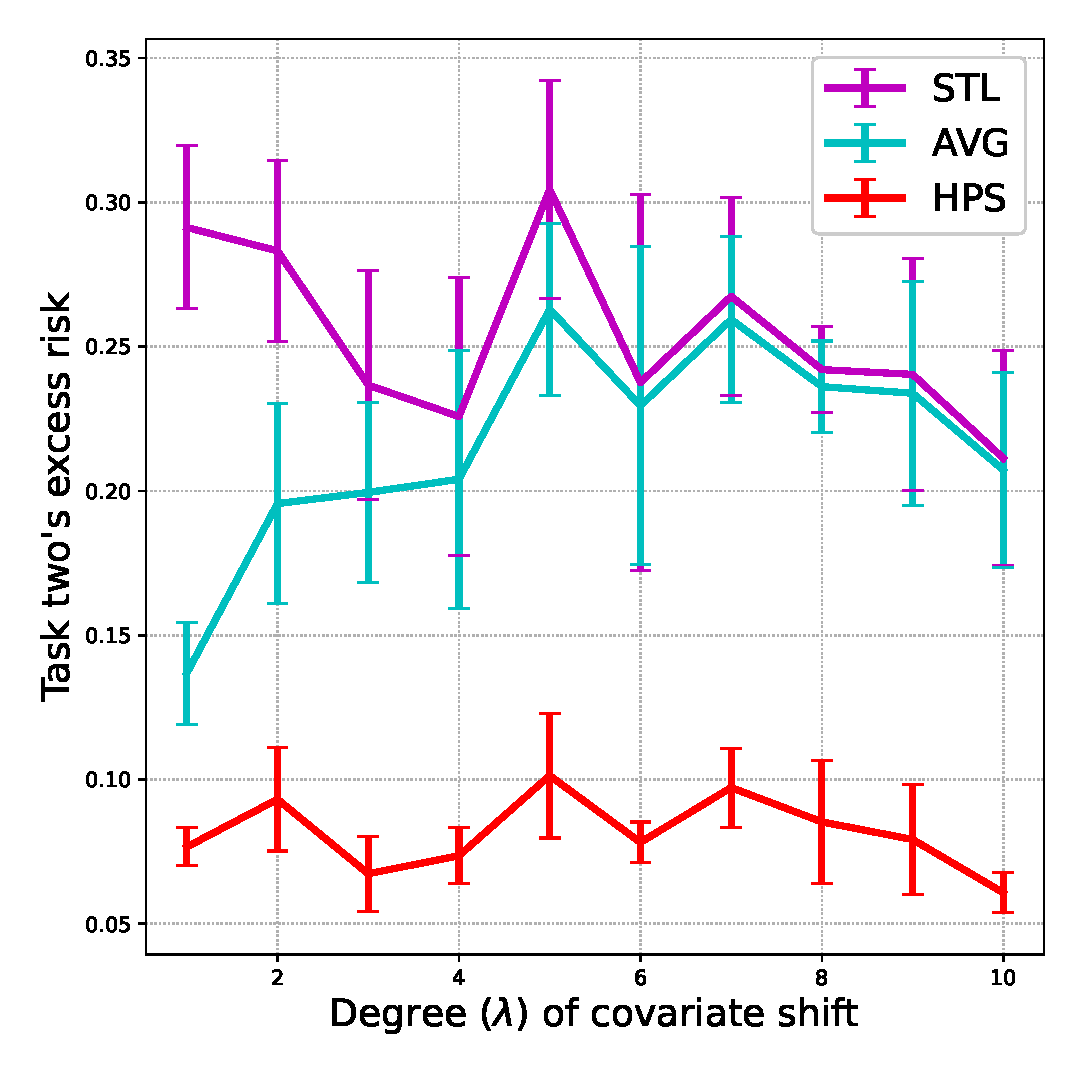
\includegraphics[width=0.95\textwidth]{figures/compare_risk_covariate_shift.eps}
		\caption{Covariate shift}
		\label{fig_sec5_covariate}
	\end{subfigure}\hfill%
	\begin{subfigure}[b]{0.33\textwidth}
		\centering
		\includegraphics[width=0.95\textwidth]{figures/compare_risk_model_shift.eps}
		\caption{Model shift}
		\label{fig_sec5_model}
	\end{subfigure}\hfill%
	\begin{subfigure}[b]{0.33\textwidth}
		\centering
		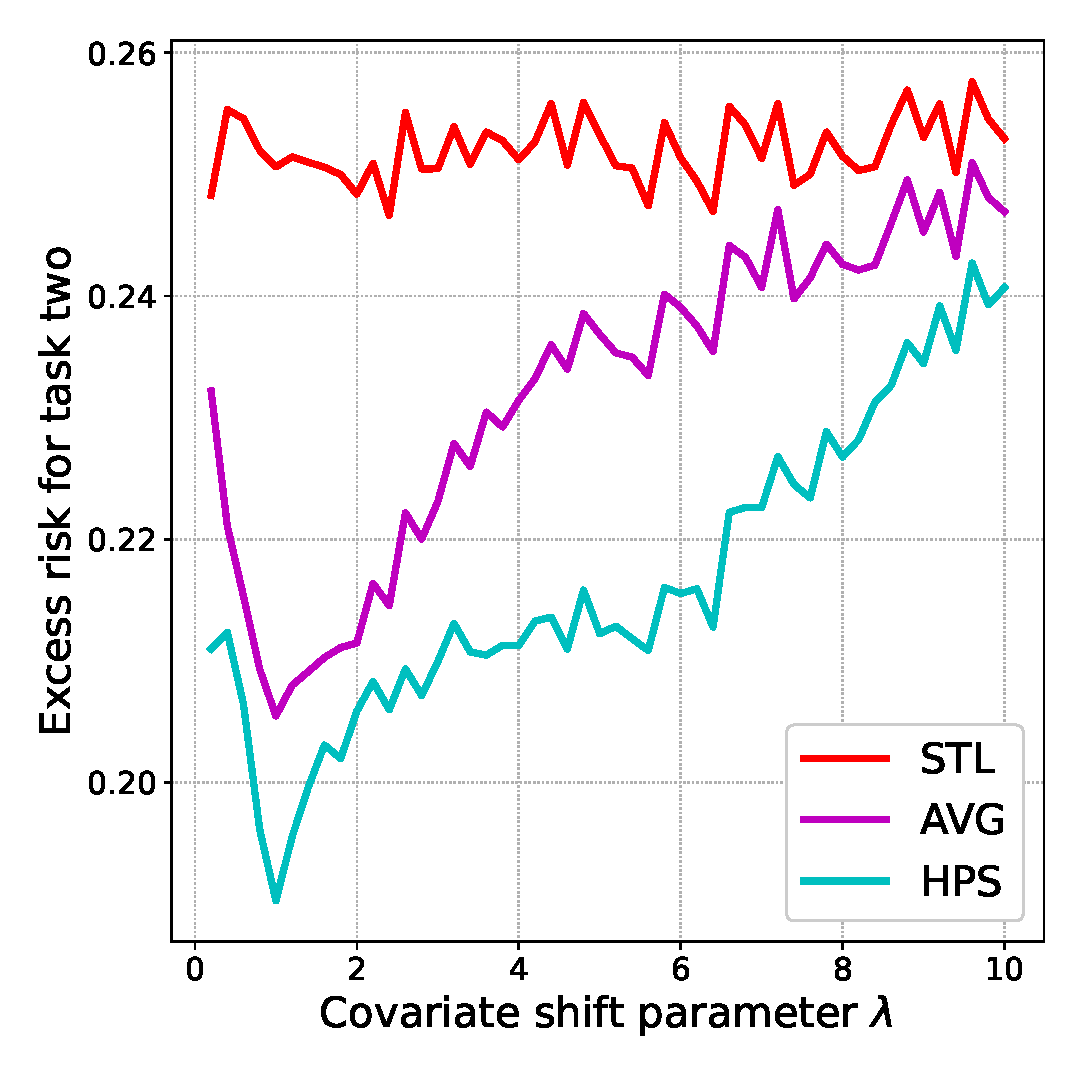
\includegraphics[width=0.95\textwidth]{figures/compare_risk_cov_model_shift.eps}
		\caption{Covariate and model shift}
		\label{fig_sec5_cov_model}
	\end{subfigure}
	\caption{We compare the empirical excess risk of HPS and several natural transfer learning estimators. We find that HPS achieves the lowest excess risk for predicting task two under (either or both) covariate and model shift. This simulation uses $p = 100, n_1 = n_2 = 200, \sigma = 1/2$. Figure \ref{fig_sec5_cov_model} uses $\lambda = 4$ for generating covariate-shifted features.}
	\label{fig_sec51}
\end{figure}

We show that HPS estimators enjoy superior empirical performance compared to several natural transfer learning estimators.
We consider the following estimators for this comparative study:
\begin{itemize}
    \item {\bf Averaging estimator (AVG):} given two tasks, take a convex combination of their OLS estimators $b \cdot \hat{\beta}^{\STL}_1 + (1 - b) \cdot \hat{\beta}^{\STL}_2$.
    \item {\bf STL estimator (STL):} simply use the OLS estimator of task two $\hat{\beta}^{\STL}_2$ without using task one's data.
    \item {\bf Transfer learning estimator (TL):} simply use the OLS estimator of task one $\hat{\beta}^{\STL}_1$ without using task two's data.
\end{itemize}
The parameter $b$ in the averaging estimator is optimized using a validation set of the same size as the training set.
Additionally, we extend the two-layer neural network formulation of HPS (cf. equation \eqref{eq_hps}) to a weighted objective:
$b \cdot \bignorm{X^{(1)} B A_1 - Y^{(1)}}^2 + (1 - b) \cdot  \bignorm{X^{2} B A_2 - Y^{(2)}}^2$, and optimize $b$ using the same validation set.

Figure \ref{fig_sec51} shows the result under (either or both) covariate and model shifts.
Figure \ref{fig_sec5_covariate} uses the same data generating process as Figure \ref{fig_sec31}.
Figure \ref{fig_sec5_model} uses the same data generating process as Figure \ref{fig_sec3_model_shift}.
Figure \ref{fig_sec5_cov_model} combines both by generating covariate-shifted features and different linear models for each dataset.
For reach run, we average the result over 100 random seeds because of high variance from the small sample sizes.
We find that HPS outperforms all the other estimators in this simulation (the result for the TL estimator is worse than STL and is omitted from the figure).

%\subsection{Implications for regression methods}


\subsection{Implications for neural networks}

\begin{wrapfigure}[12]{r}{0.3\textwidth}
	\vspace{-0.35in}
	\begin{center}
		\includegraphics[width=0.27\textwidth]{figures/mtl_model_arch.pdf}
	\end{center}
	\vspace{-0.28in}
	\caption{A hard parameter sharing neural network.}
	\label{fig_intro_arch}
\end{wrapfigure}
We conduct further studies of HPS for text classification tasks.
We consider six datasets for predicting movie review sentiment (MR and SST), sentence subjectivity (SUBJ), customer review sentiment (CR), question types (TREC), and polarity of a phrase (MPQA).\footnote{The datasets can be downloaded at \url{https://github.com/harvardnlp/sent-conv-torch/tree/master/data}. Further statistics of each dataset can also be found following the link.}
%\cite{pang2005seeing,socher2013recursive}
%\cite{pang2004sentimental}
%\cite{pang2004sentimental}
%\cite{pang2004sentimental}
%\cite{pang2004sentimental}
% \cite{lei2018simple}
%The question is to predict positive or negative sentiment expressed in the text.
We learn a hard parameter sharing model that consists of a word embedding layer using GloVe \cite{pennington2014glove}, followed by a shared feature representation layer.\footnote{The GloVe word vectors can be downloaded at \url{https://nlp.stanford.edu/projects/glove/}.}
A separate output layer is used for predicting the labels of each dataset.
We evaluate on three possibilities of feature representation layers including LSTM, MLP, and CNN, as implemented by PyTorch.\footnote{\url{pytorch} Before the MLP layer, we apply an average pooling layer over the embedding of every word in the sentence.}
See Figure \ref{fig_intro_arch} for an illustration of the network architecture.

\paragraph{Covariate alignment for mitigating covariate shift.}
We apply our theoretical insights to conduct detailed analysis of a covariate alignment procedure proposed by \citet{WZR20}.
The idea of this procedure is to insert an ``alignment'' module (or matrix) between every input $X_i$ and the shared module $B$.
During training, the entire network is optimized together with this alignment module (see \citet{WZR20} for more details about the implementation).

Our hypothesis is that as $n_1 / n_2$ increases, performing covariate alignment leads to larger accuracy improvement over the baseline HPS.
Recall from Claim \ref{prop_covariate} that covariate shift between the data source and the target task worsens the performance of HPS.
The effect is further exacerbated when the sample size of the data source is larger than the target task.
%This observation highlights the need for mitigating covariate shift when $n_1 / n_2$ increases.
To verify the hypothesis, we conduct multi-task training over all 15 pairwise tasks (among the six datasets).
We measure the average accuracy improvement from performing covariance alignment vs. HPS (trained using stochastic gradient descent (SGD)) over the 15 task pairs.
Figure \ref{fig_ab_cov} confirms our hypothesis.
We observe that covariate alignment achieves up to 4\% accuracy improvement as $n_1 / n_2$ increases.
%We fix task two's sample size at $1,000$, and increase task one's sample size from $1,000$ to $3,000$.


%\textit{Predicting transfer effect via STL results.}
%We show that the single-task based metric proposed in Section \ref{sec_similarity} can predict positive or negative transfer in MTL.
%A common challenge in the study of MTL is that the results can be hard to understand.
%It is difficult to predict when MTL performs well without running extensive trials.
%Our insight is that we can use STL results to help understand MTL results.
%Table \ref{tab:mtl_better_than_stl} shows the result on both the sentiment analysis and the ChestX-ray14 tasks.
%We find that using a threshold of $\tau = 0.1$, the STL results correctly predict positive or negative transfer with $75.6\%$ precision and $38.8\%$ recall among $30$ times $5$ (random seeds) task pairs!
%We observe similar results for $91$ task pairs from the ChestX-ray14 dataset.
%The results show that STL results are indicative of MTL results.

\paragraph{Progressive training for mitigating model shift.}
Inspired by our theoretical analysis, we propose a progressive training procedure that reduces the computational cost of learning HPS networks.
To motivate this procedure, we first conduct an experiment similar to Figure \ref{fig_sec3_model_transition}) but using the text classification datasets instead.
In Figure \ref{fig_ab_data}, we find that for multiple pairs of datasets, increasing $n_1$ improves task two's test accuracy initially, but hurts eventually.

These examples and the ones in Figure \ref{fig_sec3_model_transition} suggest a natural progressive training procedure that increases $n_1$ progressively until performance drops.
Concretely, we first divide the training data into $S$ batches.
Then, we progress in $S$ stages during training. During each stage, we progressively add one more minibatch of data from the data source(s).
During each stage, we run SGD for $T$ epochs using only the available minibatches of data.
We terminate once task two's validation accuracy drops compared to the previous round's result or reaches a desired threshold $\tau$.
See Algorithm \ref{alg_inc_train} for the complete procedure.
As an example, this procedure will terminate at the optimal value of $n_1$ if applied to the settings of Figures  \ref{fig_sec3_model_transition} and \ref{fig_ab_data}.
In light of these observations, our hypothesis is that this procedure requires a lower computational cost compared to SGD.
%For example, if the procedure terminates at 30\% of all batches, then SGD only passes over 30\% of its data, whereas standard round-robin training passes over 100\% of task one's data.

\begin{figure}[!t]
	\begin{subfigure}[t]{0.5\textwidth}
		\centering
		\vspace{0pt}
		\includegraphics[width=0.8\textwidth]{figures/fig3b.pdf}
		\caption{Covariate alignment under varying sample sizes}
		\label{fig_ab_cov}
	\end{subfigure}\hfill
	\begin{subfigure}[t]{0.5\textwidth}
		\centering
		\vspace{0pt}
		\includegraphics[width=0.8\textwidth]{figures/fig3a.pdf}
		\caption{Information transfer under varying sample sizes}
		\label{fig_ab_data}
	\end{subfigure}
	\caption{
	We extend some of our theoretical observations to text classification tasks using HPS neural networks.
	Figure \ref{fig_ab_cov} shows that covariance alignment improves the task two's test accuracy more for larger sample size ratio $n_1 / n_2$.
 	Figure \ref{fig_ab_data} shows that task one provides a positive transfer to task two in HPS only for a restricted range of $n_1$ (similar to Figure \ref{fig_sec3_model_transition}).
    Both experiments fixes $n_2 = 1000$ while varying $n_1$ from $100$ to $3000$.
	The $y$-axis measures task two's test accuracy using HPS subtracted by its test accuracy without using task one's data.}
	\label{fig_text}
\end{figure}


\begin{algorithm}[!h]
	\caption{Progressive training of hard parameter sharing networks}
	\label{alg_inc_train}
	\begin{algorithmic}[1]
		\Input Two tasks $(X^{(1)}, Y^{(1)})$ and $(X^{(2)}, Y^{(2)})$, divided into a training, validation, and test set.
		\Param A shared module $B$, and output layers $A_1, A_2$.
		\Req Number of batches $S$, epochs $T$, a threshold $\tau\in(0,1)$.
		\Output The trained modules $B, A_2$ optimized for task two.
		\State Divide the training set of $(X^{(1)}, Y^{(1)})$ randomly into $S$ batches: $(x^{(1)}, y^{(1)}), \dots, (x^{(S)}, y^{(S)})$.
		\For{$i = 1,\dots, S$}
		\For{$j = 1,\dots, T$}
		\State Minimize the cross-entropy loss of $B, A_1, A_2$ on  $\set{(x^{(k)}, y^{(k))}}_{k=1}^i$ and the training set of $(X^{(2)}, Y^{(2)})$ using SGD.
		\EndFor
		\State Let $a_i$ be the current validation accuracy for task two.
		\If{$a_i < a_{i-1}$ or $a_i > \tau$}
		\State \textbf{break}
		\EndIf
		\EndFor
	\end{algorithmic}
\end{algorithm}

\smallskip
\begin{wrapfigure}[10]{r}{0.26\textwidth}
	\vspace{-0.15in}
	\centering
	\begin{tabular}{c c c}
		\toprule
		Models & Relative cost \\
		\midrule
		{\bf CNN}  & 30\% \\
		{\bf LSTM} & 35\% \\
		{\bf MLP}  & 31\%  \\
		\bottomrule
		\end{tabular}
		\captionof{table}{The computational cost of running Algorithm \ref{alg_inc_train} relative to the cost of running SGD.}
		\label{tab:taskonomy}
	\label{fig_intro_arch}
\end{wrapfigure}
We evaluate Algorithm \ref{alg_inc_train} in two scenarios.
First, we consider transferring from single data source to a target task.
We evaluate over all $15$ two-task pairs.
We find that when averaged over all the pairs, our procedure requires less than $35\%$ of the computational cost relative to SGD while reaching the same level of test accuracy for predicting task two.
Second, we consider transferring from multiple data sources.
We use all six datasets as data sources to help predict every other task---that is, we measure the average accuracy of predicting all six tasks.
We find that a similar progressive training style procedure requires less than $35\%$ of the computational cost (relative to the cost of running SGD) for reaching the same average test accuracy of SGD.

\medskip
\noindent\textit{Further details.}
Algorithm \ref{alg_inc_train} uses SGD during the minimization step.
We randomly shuffle the data of both tasks and apply SGD on the shuffled data.
For the two-task experiment, we set $\tau$ to be task two's (STL) test accuracy trained without using any other task's data.
%We include all of task two's data and progressively add task one's data using the procedure described above.
%As a result, once Algorithm \ref{alg_inc_train} terminates, task two's test accuracy is at least $\tau$.
For the six-task experiment, We set $\tau$ to be the average test accuracy of all six tasks trained using all tasks' data.
We include the data from all tasks except SST. For SST, we progressively increasing its sample size similar to Algorithm \ref{alg_inc_train}.



%\begin{figure}[!t]
%	\centering
%	\begin{subfigure}[b]{0.5\textwidth}
%		\centering
%		\includegraphics[width=0.5\textwidth]{figures/ratio_alignment_norm_diff_all.pdf}
%		\caption{Averaged over all 16 task pairs}
%		\label{fig_ab_cov}
%	\end{subfigure}\hfill
%	\begin{subfigure}[b]{0.5\textwidth}
%		\centering
%		\includegraphics[width=0.5\textwidth]{figures/ratio_alignment_norm_trec_cr_lstm.pdf}
%		\caption{An example task pair}
%		\label{fig_cov_a}
%	\end{subfigure}
%	\caption{ (TREC and CR)}
%\end{figure}

%\textbf{Further results of the covariance alignment procedure.}
%Our results in Figure \ref{fig_ab_cov} are averaged over all the task pairs.
%In Figure \ref{fig_covariate_app}, we show two task pairs as examples.
%In Figure \ref{fig_cov_a}, we observe that for the particular task pair, covariance alignment provides more significant gains when the sample ratio is large.
%In Figure \ref{fig_cov_b}, we observe that covariance alignment does not always improve over the baseline multi-task learning model.
%One explanation is that MR and SST are similar tasks, hence adding the alignment module is unnecessary.
%An interesting question is to understand when adding the alignment module benefits the multi-task learning model.
%We leave this question for future work.
%Note: For text classification tasks, the source task training data size ranges from 500 to 1,500 and target task training data size is 1000; For ChestX-ray14,

%\begin{figure}[!h]
%	\centering
%	\begin{subfigure}[b]{0.48\textwidth}
%		\centering
%		\includegraphics[width=0.7\textwidth]{figures/ratio_alignment_norm_trec_cr_lstm.pdf}
%		\caption{Task pair TREC and CR}
%		\label{fig_cov_a}
%	\end{subfigure}\hfill
%		\begin{subfigure}[b]{0.48\textwidth}
%		\centering
%		\includegraphics[width=0.7\textwidth]{figures/ratio_alignment_mr_sst_lstm.pdf}
%		\caption{Task pair MR and SST}
%			\label{fig_cov_b}
%	\end{subfigure}
%	\caption{(a) For the task pair TREC and CR, adding the covariance alignment procedure provides more improvement when the source/target sample ratio is large.
%	(b) For the task pair MR and SST, adding the covariance alignment procedure hurts performance.
%	One explanation is that MR and SST are similar tasks, hence adding the alignment module is unnecessary.}
%	\label{fig_covariate_app}
%\end{figure}
    \section{Transferring from multiple source tasks}\label{sec_same}

%We begin by considering the case where all tasks have the same sample size and feature covariates, that is, $n_i = n$ and $X^{(i)} = X\in\real^{n\times p}$ for all $i = 1, \dots, t$.
%We provide a sharp generalization error bound of hard parameter sharing estimators.

Hard parameter sharing is a commonly used architecture in multi-task learning. However, there have been few theoretical results on the performance of the HPS estimators in high-dimensional multi-task learning. In this section, we extend our results on the predication loss of the HPS estimator to a multi-task linear regression, where all tasks have the same covariates. We make this extension for the following reasons. First, its restriction to the two-task case provides a rare example where the output layers $A_1$ and $A_2$ can be characterized exactly. Second, the proof of the multi-task case is no harder than the two-task case, but it can provide much clearer geometric intuition  as we will discuss below. Third, the corresponding multi-task setting is prevalent in applications of multi-task learning to image classification, where there are multiple prediction labels/tasks for every image \cite{chexnet17,EA20}. Finally, it provides useful insights into a more general theory of multi-task learning, which we will explore in greater details in future works.
%It is not hard to extend the above result to the cases with more than two tasks. {\cor For the general case, we study them in a future work.}

%Suppose we have $t$ datasets.
%For each dataset $i$ from $1$ to $t$, let $n_i$ denote its sample size.
%Let $X^{(i)} \in \real^{n_i \times p}$ denote dataset $i$'s feature covariates.
%We assume that the label vector $Y^{(i)} \in \real^{n_i}$ for $X^{(i)}$ follows a linear model plus random noise.
%We study the standard hard parameter sharing architecture:
%a shared feature representation layer $B\in\real^{p\times r}$ for all datasets and a separate output layer $A_i \in \real^r$ for every dataset $i$.
%See Figure \ref{fig_intro_arch} for an illustration.
%The width of $B$, denoted by $r$, plays an important role in regularization.
%As observed in Proposition 1 of \cite{WZR20}, if $r \ge t$, there is no regularization effect.
%Hence, we assume that $r < t$ in our study.
%For example, when there are only two tasks, $r = 1$ and $B$ reduces to a vector whereas $W_1, W_2$ become scalars.
%We study the following minimization problem:
%	\item Separate each dataset $(X_i, Y_i)$ randomly into a training set $(X_i^{tr}, Y_i^{tr})$ and a validation set $(X_i^{val}, Y_i^{val})$.
%	The size of each set is described below.
%	\item Learn the shared layer $B$: minimize the training loss over $B$ and $W_1, \dots, W_t$, leading to a local minimum of $B$ that depends on $W_1, \dots, W_t$, denoted by $\hat{B} = \hat{B}(W_1, \dots, W_t)$.
%\vspace{-0.1in}
%\begin{align}\label{eq_mtl}
%			f(A, B) = \sum_{i=1}^t \norm{X^{(i)} B A_i - Y^{(i)}}^2,
%\end{align}
%\vspace{-0.05in}
%where $A = [A_1, A_2, \dots, A_t] \in \real^{r \times t}$.

\vspace{5pt}
\noindent\textbf{Multi-task setting.} Suppose we have $t$ datasets whose sample sizes are all equal to $n$ and whose feature covariates are all equal to $X \in \real^{n \times p}$. The label vector of the $i$-th task follows a linear model
$$Y^{(i)} = X \beta^{(i)} + \varepsilon^{(i)},\quad i=1,2,\cdots, t.$$
We assume that $X=Z\Sigma^{1/2}$ is a random matrix satisfying the same assumption as $X^{(2)}$ in Assumption \ref{assm_big1}, that is, $Z$ is an $n\times p$ random matrix with i.i.d. entries satisfying (\ref{assm1}) and \eqref{conditionA2}, $\Sig$ is a deterministic positive definite symmetric matrix satisfying \eqref{eigen} and \eqref{assm3}, and $\rho:=n/p$ satisfies \eqref{assm2}. $\varepsilon^{(i)} \in \real^{n}$, $i=1,2,\cdots, t$, are independent random vectors with i.i.d entries of mean zero, variance $\sigma^2$, and bounded moments as in \eqref{eq_highmoments}. Finally, $X$, $\ve^{(i)}$ and $\beta^{(i)}$, $i=1,2,\cdots, t$, are all  independent from each other.

%\begin{enumerate}
%	\item $X = Z \Sigma^{1/2} \in \real^{n\times p}$ for a positive semidefinite matrix $\Sigma\in \R^{p\times p}$, and every entry of $Z \in \real^{n \times p}$ is drawn independently from a one dimensional distribution with zero mean, unit variance, and constant $\varphi$-th moment for a fixed $\varphi > 4$.
%	\item every entry of $\varepsilon^{(i)} \in \real^{n \times t}$ is drawn indepdently from a one dimensional distribution with zero mean, variance $\sigma^2$, and bounded moment up to any order.\footnote{There exists a fixed function $C: \mathbb{N} \rightarrow \real^+$ such that for any $k \in \N$, the $k$-th moment is bounded by $C(k)$.}
%\end{enumerate}


	To define the HPS parameter for the above setting, we study the following minimization problem % \eqref{eq_tsl} becomes
	\begin{align}
		f(A, B) = \sum_{j=1}^t \bignorm{X B A_j - Y^{(j)}}^2, \label{eq_mtl_same_cov}
	\end{align}
	where $B \in \real^{p \times r}$ is a rank-$r$ shared feature representation layer, and $A := [A_1, A_2, \dots, A_t] \in \real^{r \times t}$ with $A_i \in \R^r$ being a separate output layer for task $i$. %Recall that $r$ is the width of $B$.
We will focus on cases with $r < t$, because otherwise the global minimum of $f(A, B)$ reduces to single-task learning (cf. Proposition 1 of \cite{WZR20}).

	%If $r\ge t$, then it is trivial to observe that we can always choose the parameters $A$ and $B$ such that $BA_i$ can fit any parameter $\beta^{(i)}\in \R^p$, which leads to a vanishing predication loss. Hence we only consider the case with $r<t$. \FY{Correct it if the reason is wrong.}

	For the optimization objective  in \eqref{eq_mtl_same_cov}, using the local optimality condition over $B$, that is, $\frac{\partial f}{\partial B} = 0$, we obtain $\hat{B}$ as a function of $A$:
	\begin{align}
		\hat{B}(A) %&\define (X^{\top}X)^{-1} X^{\top} \bigbrace{\sum_{j=1}^t Y^{(j)} A_j^{\top}} (A  A^{\top})^{+} \nonumber \\
		&= (X^{\top} X)^{-1} X^{\top} Y A^{\top} (AA^{\top})^{+}, \label{eq_Bhat}
	\end{align}
	where $Y := [Y^{(1)}, Y^{(2)}, \dots, Y^{(t)}]$ and $(AA^{\top})^{+}$ denotes the pseudoinverse of $AA^{\top}$.
	%Here we have used that $X^{\top}X$ is invertible since $n > \rho \cdot p$ and $\rho > 1$ (cf. Fact \ref{fact_minv}).
	%\FY{Is $\dag$ a standard notation? It is a bad notation at least for me because $\dag$ is more often used as Hermitian conjugate. Wiki page uses $(AA^{\top})^{+}$ for pseudo-inverse.}
	Plugging $\hat{B}(A)$ into equation \eqref{eq_mtl_same_cov}, we obtain the following objective that only depends on $A$ (in matrix notation):
	\begin{align}\label{eq_mtl_output_layer}
		g(A) = \bignormFro{X (X^{\top}X)^{-1}X^{\top} Y A^{\top} (AA^{\top})^{+} A - Y}^2.
	\end{align}
%	Note that $A^{\top} (AA^{\top})^{+} A$ is a projection onto the subspace spanned by the rows of $A$. For simplicity, we write it into the form
%	$$A^{\top} (AA^{\top})^{+} A= U_A U_A^\top,$$
%	where $U_A \in \R^{t\times r}$ is a $t\times r$ partial orthonormal matrix (i.e. $U_A^\top U_A=\id_{r\times r}$). Hence we also denote the function $g(A)$ by $g(U_A)$.
Let $\hat A$ be the global minimizer of $g(A)$. Then $(\hat A,\hat B(\hat A))$ is the global minimizer of $f(A,B)$. We define the HPS estimator for task $i$ as $\hat \beta_i^{\MTL} := \hat B(\hat A) \hat A_i,$
%For an estimator $\hat{\beta}_i$ of task $i$, we are interested in
and its (out-of-sample) prediction loss as
\be\label{ith_loss} L_i(\hat{\beta}_i^{\MTL}) = \bignorm{\Sigma^{1/2} \left(\hat{\beta_i}^{\MTL} - \beta^{(i)}\right)}^2. \ee


Our main result of this section, Theorem \ref{thm_many_tasks}, shows that hard parameter sharing essentially approximates all tasks through a rank-$r$ subspace. To formalize this geometric intuition, as in the two-task case, we introduce the matrix $B^\star \define [{\beta}^{(1)},{\beta}^{(2)},\dots,{\beta}^{(t)}] \in \real^{p\times t}$ formed by the linear model parameters of all the $t$ tasks.
Let $A^{\star} {A^{\star}}^{\top}$ denote the best rank-$r$ subspace approximation of ${B^{\star}}^\top\Sigma B^{\star}$ (which can be regarded as the covariance of the task labels):
\begin{align}\label{eq_A_star}
	A^{\star} \define \argmin_{U\in\real^{t\times r} : U^{\top} U = \id_{r\times r}} \inner{U U^{\top}} {{B^{\star}}^{\top} \Sigma B^{\star}},
\end{align}
where $\langle \cdot ,\cdot \rangle $ denotes the Frobenius inner product between two matrices.
 To ensure that $A^{\star}$ is unique, we assume that the $r$-th largest eigenvalue of ${B^\star}^\top \Sigma B^\star$ is strictly larger than the $(r+1)$-th largest eigenvalue. Otherwise, $A^{\star}$ is not well-defined and Theorem \ref{thm_many_tasks} will give a null result.
 %$\lambda_{r+1}({B^\star}^\top \Sigma B^\star)$ is strictly smaller than $\lambda_{r}({B^\star}^\top \Sigma B^\star)$.
Let $a_i^{\star}:= A^{\star}{A^{\star}}^{\top} e_i \in\real^r$ denote the $i$-th column of $A^{\star}{A^{\star}}^{\top}$, where $e_i$ is the standard basis unit vector along $i$-th direction. Then we have the following result.


% $B^{\star} A^{\star} {A^{\star}}^{\top}$.
%Let $(\hat{A}, \hat{B})$ be the global minimizer of $f(A, B)$.
%Recall that the HPS estimator is defined as $\hat{\beta}_i^{\MTL} = \hat{B} \hat{A}_i$.
%Our result is stated as follows.

\begin{theorem}\label{thm_many_tasks}
%Suppose $X=Z\Sigma^{1/2}\in \R^{n\times p}$ satisfy Assumption \ref{assm_secA1} with $\rho:=n/p>1$ being some fixed constant. Consider data models  $Y_i = X\beta_i + \varepsilon_i$, $i=1,2,\cdots, t$, where $\e_i\in \R^{n}$ are random vectors with i.i.d. entries with mean zero, variance $\sigma^2$ and all moments as in \eqref{assmAhigh}. Moreover, assume that $X$, $\beta_i$ and $\e_i$ are all independent of each other.
	%Let $n = c \cdot p$.
	%Let $X\in\real^{n\times p}$ and $Y_i = X\beta_i + \varepsilon_i$, for $i = 1,\dots,k$.
%	Consider $t$ data models $Y_i = X\beta_i + \varepsilon_i$, $i=1,2,\cdots, t$, where $X$ has covariance matrix $\Sigma$, and the entries of $\e_i$ are i.i.d. with mean zero and variance $\sigma^2$.gT
	%that satisfy Assumption \ref{assm_secA2} in the appendix.
	%Assume that $n > \rho \cdot p$ for a fixed constant $\rho > 1$.
	%Let $c_{\varphi}$ be any fixed value within $(0, \frac{\varphi-4}{2\varphi})$.
%	Let $L(B^{\star}a_i^{\star}): = \norm{\Sigma^{1/2} (B^{\star} a_i^{\star}- \beta^{(i)})}^2$.
%Suppose $X\in \R^{n\times p}$ is an $n\times p$ random matrix satisfying the same assumptions as $X^{(1)}$ and $X^{(2)}$ in Assumption \ref{assm_big1}, and $\rho:=n/p$ satisfies \eqref{assm2}.
Suppose the above multi-task setting holds. Let $c>0$ be an arbitrary (small) constant. Then for any task $i = 1,  \cdots, t$, we have that with high probability,
\be\label{minimizer_beta}
\left\|  \hat A^{\top} (\hat A\hat A^{\top})^{+} \hat A - A^\star {A^\star}^\top\right\|_F  \le \left[ \frac{ n^{-1/2+2/\varphi+c}  \|{B^{\star}}^{\top}\Sigma B^{\star}\|  + n^{-1/2+c} \sigma^2 }{\lambda_r - \lambda_{r+1} }\right]^{1/2} ,
\ee
where $\lambda_r $ and $\lambda_{r+1}$ are respectively the $r$-th and $(r+1)$-th largest eigenvalues of ${B^\star}^\top\Sigma B^\star$. Moreover, the prediction loss of the HPS estimator $\hat{\beta}_i^{\MTL}$ satisfies that  with high probability,
	\begin{align}
		& \bigabs{L_i(\hat{\beta}_i^{\MTL}) - L_i(B^{\star}a_i^{\star}) -\frac{p\sigma^2}{n-p}  \norm{a_i^{\star}}^2  } \nonumber\\
		& \le  \left[ \frac{  n^{-1/2+ 2/\varphi +c}   \norm{{B^\star}^\top\Sigma B^\star} +n^{-1/2+c}  \sigma^2} {\lambda_r  - \lambda_{r+1} }\right]^{1/2}  \left(\norm{{B^\star}^\top\Sigma B^\star}+  \sigma^2\right). \label{Li_multi1}
		%\le n^{-\frac{c_{\varphi}}2} \cdot \frac{\bigbrace{ \norm{\Sigma^{1/2} B^{\star}}^2+  \sigma^2} \cdot (\bignormFro{\Sigma^{1/2} B^{\star}}^2 + \sigma^2 t)} {\lambda_r ({B^\star}^\top \Sigma B^\star)- \lambda_{r+1}({B^\star}^\top \Sigma B^\star)},
	\end{align}
	%where $\lambda_r({B^\star}^\top\Sigma B^\star)$ and $\lambda_{r+1}({B^\star}^\top\Sigma B^\star)$ are respectively be the $r$-th and $(r+1)$-th largest eigenvalue of ${B^\star}^\top\Sigma B^\star$.
%	where $C_1: = \frac{\bignormFro{\Sigma^{1/2} B^{\star}}^2 + \sigma^2 t}{\lambda_r ({B^\star}^\top \Sigma B^\star)- \lambda_{r+1}({B^\star}^\top \Sigma B^\star)}$. %and $C_2 :=  C_1\cdot \norm{\Sigma^{1/2} B^{\star}}$.
Finally, we have a better bound for the averaged prediction loss:  with high probability,
\begin{align}
&\left|\frac{1}{t}\sum_{i=1}^t L_i(\hat{\beta}_i^{\MTL}) - \frac1t\bignorm{\Sigma^{1/2} B^{\star} (A^\star {A^\star}^{\top} - \id_{t\times t})}_F^2 - \frac{p \sigma^2}{n-p}\cdot \frac{r}{t}  \right| \nonumber \\
 &\le n^{-1/2+2/\varphi+c}  \norm{{B^\star}^\top\Sigma B^\star}+ n^{-1/2+c}   \sigma^2 .\label{Li_multi2}
\end{align}

\end{theorem}

Recall that $\varphi$ is a constant larger than 4, hence $n^{-1/2+2/\varphi+c}$ is a negligible  factor asymptotically as long as $c$ is smaller than $1/2-2/\varphi$. Moreover, the factor $(\lambda_r - \lambda_{r+1})^{-1}$ is natural, because the best rank-$r$ subspace approximation of ${B^{\star}}^\top\Sigma B^{\star}$ is not stable when $\lambda_r $ and $\lambda_{r+1} $ are close to each other.  The bound \eqref{minimizer_beta} verifies our intuition that hard parameter sharing approximates the matrix ${B^{\star}}^\top\Sigma B^{\star}$ through a best rank-$r$ subspace. The estimate \eqref{Li_multi1}
 gives the exact asymptotic limit of $L_i(\hat{\beta}_i^{\MTL}(\hat a))$, which shows that the prediction loss of $\hat{\beta}_i^{\MTL}$ decomposes into a bias term $L_i(B^{\star} a_i^{\star})$ that measures the prediction loss of $B^{\star} a_i^{\star}$, plus a variance term that scales with $\norm{a_i^{\star}}^2$. Since $\norm{a_i^{\star}}^2\le 1$, compared with the single-task predication loss \eqref{L_STL_simple01}, the variance term always decreases for the multi-task HPS estimator. On the other hand, the bias term always increases (because the bias in single-task linear regression is zero). Hence as in the transfer learning setting, whether the HPS estimator is better than the OLS estimator depends on an intricate  {bias-variance tradeoff}.
%{\cor One direct implication of our result is that compared to STL, the variance always decreases, since STL's variance is equal to $\sigma^2 \tr[\Sigma (X^{\top} X)^{-1}]$.
%On the other hand, the bias always increases.}
We can observe a similar {bias-variance tradeoff} for the averaged predication loss in \eqref{Li_multi2} using the fact that $r<t$. Note that the estimate \eqref{Li_multi2} can be applied even when the best rank-$r$ subspace approximation of ${B^{\star}}^\top\Sigma B^{\star}$ is not unique. For all the estimates in Theorem \ref{thm_many_tasks}, we believe that their convergence rates are asymptotically tight when $n$ goes to infinity.


The proof of Theorem \ref{thm_many_tasks} will be given in Appendix  \ref{app_proof_error_same_cov} of the supplement \cite{MTL_suppl}. Moreover, by setting $t=2$ in Theorem \ref{thm_many_tasks}, we can obtain the prediction loss for the HPS estimator for the transfer learning setting where the two tasks have the same covariates  $X^{(1)}=X^{(2)}$. For the reader's convenience, we give the precise statement in Corollary \ref{thm_two_tasks}.
%Theorem \ref{thm_many_tasks} implies Theorem \ref{thm_two_tasks} as a special case with $t=2$ and $r=1$.
%In this section, we consider the setting where the two tasks have the same covariates  $X^{(1)}=X^{(2)}$.
We define $A^\star \in \R^{2}$ as the normalized eigenvector corresponding to the larger eigenvalue of the $2\times 2$ matrix
$ {B^\star}^\top \Sigma  B^\star,$ where recall that $B^\star \define [{\beta}^{(1)},{\beta}^{(2)}] \in \real^{p\times 2}$ by definition.
% is the matrix formed by the linear model parameters of the two tasks.
Without loss of generality, we assume that the two eigenvalues of ${B^\star}^\top \Sigma B^\star$ are not degenerate, so that $A^\star$ is uniquely defined. %Otherwise, Theorem \ref{thm_two_tasks} will give a null result.
In the following corollary, the estimate \eqref{minimizer_beta1} shows that the minimizer $\hat a$ is approximately equal to $A^\star(1)/A^\star(2)$, while \eqref{Li_multi0} gives the exact asymptotic limit of $L_2(\hat{\beta}_2^{\MTL}(\hat a)) $, together with an explicit convergence rate that we believe to be sharp.

\begin{corollary}\label{thm_two_tasks}
Under Assumption \ref{assm_big1}, suppose that $X^{(1)}=X^{(2)}$ and $n_1=n_2\equiv n$. Let $c>0$ be an arbitrary (small) constant. Then we have that with high probability,
\be\label{minimizer_beta1}
\left\| u_{\hat a}u_{\hat a}^\top - A^\star {A^\star}^\top\right\|_F  \le  \left[\frac{ n^{-1/2+2/\varphi+c}  \|{B^{\star}}^{\top}\Sigma B^{\star}\|  + n^{-1/2+c} \sigma^2 }{\lambda_1 - \lambda_{2} } \right]^{1/2},
\ee
where $u_{\hat a}$ is the unit vector defined as
$ u_{\hat a}:= \frac1{\hat a^2 +1} \begin{pmatrix} {\hat a}\\ 1\end{pmatrix},$ and $\lambda_1 $ and $\lambda_{2}$ are respectively the larger and smaller eigenvalues of ${B^\star}^\top\Sigma B^\star$.
%for task 2,  % over the randomness of the input,
Moreover, the prediction loss of the HPS estimator satisfies that with high probability,
	\begin{align}
		& \bigabs{L_2(\hat{\beta}_2^{\MTL}(\hat a)) - \left\|(\Sigma^{(2)})^{1/2} \left(A^\star(2) \cdot B^{\star}A^{\star}  - \beta^{(2)}\right)\right\|^2  - |A^\star(2)|^2  \frac{p\sigma^2}{n-p} } \nonumber\\
		& \le  \left[  \frac{  n^{-1/2+2/\varphi+c} \|{B^{\star}}^{\top}\Sigma B^{\star}\|+n^{-1/2+c} \sigma^2} {\lambda_1  - \lambda_2 }\right]^{1/2}   \left(\norm{\Sigma^{1/2} B^{\star}}^2+  \sigma^2\right), \label{Li_multi0}
		%\le n^{-\frac{c_{\varphi}}2} \cdot \frac{\bigbrace{ \norm{\Sigma^{1/2} B^{\star}}^2+  \sigma^2} \cdot (\bignormFro{\Sigma^{1/2} B^{\star}}^2 + \sigma^2 t)} {\lambda_r ({B^\star}^\top \Sigma B^\star)- \lambda_{r+1}({B^\star}^\top \Sigma B^\star)},
	\end{align}
	 where $A^\star(2)$ denotes the second entry of $A^\star$.
	 \end{corollary}

%The estimate \eqref{minimizer_beta1} shows that the minimizer $\hat a$ is approximately equal to $A^\star(1)/A^\star(2)$, while \eqref{Li_multi0} gives the exact asymptotic limit of $L_2(\hat{\beta}_2^{\MTL}(\hat a)) $, together with an explicit convergence rate that we believe to be sharp.


%It is not hard to extend the above result to the cases with more than two tasks. We make this extension for the following reasons. First, it provides a clearer geometric intuition than the two-task setting as we will discuss below. Second, the corresponding multi-task setting is prevalent in applications of multi-task learning to image classification, where there are multiple prediction labels/tasks for every image \cite{chexnet17,EA20}. Finally, it provides useful insights into a more general theory of multi-task learning, which we will explore in greater details in future works.

%We consider an arbitrary local minimum $B, W_1, \dots, W_2$ of the optimization objective.
%We extend the bias-variance decomposition from the two-task case to the multiple-task case.
%We observe that the expected prediction loss of $\hat{\beta}_t^{\MTL}$ conditional on $X$ consists of a bias and a variance equation as follows
%\begin{align}
%	\exarg{\varepsilon_1, \dots, \varepsilon_t}{L(\hat{\beta}_t^{\MTL}) \mid X}
%	=& \bignorm{\Sigma^{1/2} \bigbrace{B^{\star} \cW^{\top} (\cW \cW^{\top})^{-1} W_t - \beta_t}}^2 \label{eq_bias_multiple} \\
%	&+ \sigma^2 \cdot (W_t^{\top} (\cW \cW^{\top})^{-1} W_t) \cdot \bigtr{\Sigma (X^{\top} X)^{-1}} \label{eq_var_multiple}
%\end{align}
%One can see that equation \eqref{eq_bias_multiple} is the bias of the multi-task learning estimator and equation \eqref{eq_var_multiple} is its variance.
%Compared to the prediction loss of single-task learning (cf. equation \eqref{eq_var_stl}), we observe that the variance equation \eqref{eq_var_multiple} is always smaller because $W_t^{\top} (\cW \cW^{\top})^{-1} W_t \le 1$.
%On the other hand, the bias equation \eqref{eq_bias_multiple} is always larger because of the difference between the task models.
%We show the generalization error of hard parameter sharing estimators.
%Before stating the result, we define the following notations.




%The key step for proving Theorem \ref{thm_many_tasks} is a characterization of $f(A, B)$'s global minimizer.
%\medskip
%
%\noindent\textbf{Comparison to single-task learning (STL).}
%Theorem \ref{thm_many_tasks} provides a sharp generalization error bound that is asymptotically tight when $n$ goes to infinity.
%%The limiting loss of hard parameter sharing consists of two parts, a bias term $L(B^{\star} a_i^{\star})$ that measures the error of $B^{\star} a_i^{\star}$, and a variance term that scales with noise variance $\sigma^2$.
%%	Our result implies that the variance of hard parameter sharing is always smaller than single-task learning.
%%	This is because	STL's variance is equal to $\frac{\sigma^2 \cdot p} {n - p}$ by Fact \ref{lem_minv}, and $\norm{a_i^{\star}}^2 \le 1$ since the spectral norm of $U_r$, which is a projection matrix, is at most one.
%One direct implication of our result is that compared to STL, the variance always decreases, since STL's variance is equal to $\sigma^2 \tr[\Sigma (X^{\top} X)^{-1}]$.
%On the other hand, the bias always increases.


%\FY{add simulations to check our results; discuss motivations and possible applications}
\iffalse
In this paper, we consider a natural extension of the estimator $\hat \beta^{\rm{TL}} $, that is, the \emph{hard parameter sharing} (HPS) estimator, which has been a standard type of estimator in multi-task learning \FY{citations}. More precisely, we study the following HPS architecture: a shared feature representation layer $B\in\real^{p}$ for all datasets and a separate output layer $A_i \in \real$ for every dataset $i$. Then we study the following minimization problem:
\begin{align}\label{eq_tsl}
			f(A, B) = \norm{X^{(1)} B A_1 - Y^{(1)}}^2 + \norm{X^{(2)} B A_2 - Y^{(2)}}^2,
\end{align}
where we abbreviate $A = [A_1, A_2]$. Let $(\hat{A}, \hat{B})$ be the minimizer of $f(A, B)$. We define the hard parameter sharing (HPS) estimator for task $i$ as
\be\label{def_HPS}\hat{\beta}_i^{\MTL} = \hat{B} \hat{A}_i,\quad i=1,2.\ee
Note that $\hat \beta^{\rm{TL}}$ is a special case of $\hat{\beta}_i^{\MTL}$ by setting $A_1=A_2=1$.

For the optimization objective $f(A, B)$ in \eqref{eq_tsl}, using the local optimality condition $\frac{\partial f}{\partial B} = 0$, we can solve that
	\begin{align}
		\hat{B} = A_2^{-1} \hat \Sigma(a)^{-1} \left[a (X^{(1))})^{\top}Y^{(1)} +  (X^{(2)})^{\top}Y^{(2)}\right], \label{eq_Bhat_2task} %\\
		%&= (B^\star A ^{\top}) (A A^{\top})^{-1} + (X^{\top}X)^{-1}X^{\top}   \bigbrace{\sum_{j=1}^t \varepsilon_i A_i^{\top}} (A  A^{\top})^{-1}.
	\end{align}
where we denote $a:=A_1/A_2$ and $\hat \Sigma(a):= a^2 (X^{(1)})^\top X^{(1)}  + (X^{(2)})^\top X^{(2)}$.
Applying $\hat B$ to equation \eqref{eq_tsl}, we obtain an objective that only depends on $a $ as follows %\HZ{$A$ has been used to denote the output layers. Could you replace $A$ with another symbol (say $x$)?}
 \begin{align}
		 g(a) \define & \left\| X^{(1)} \hat\Sigma(a)^{-1} (X^{(2)})^\top X^{(2)} (a\beta^{(2)}-\beta^{(1)}) \right. \nonumber\\
			& \left. + \left(a^2 X^{(1)}\hat \Sigma(a)^{-1} (X^{(1)})^\top-\id_{n_1\times n_1}\right)\epsilon^{(1)}+ a X^{(1)}\hat \Sigma(a)^{-1} (X^{(2)})^\top \epsilon^{(2)} \right\|^2 \nonumber\\
		   +& \left\| X^{(2)} \hat \Sigma(a)^{-1} (X^{(1)})^\top X^{(1)} (a\beta^{(1)}-a^2\beta^{(2)}) \right. \nonumber\\
		  &\left.+ \left(X^{(2)}\hat\Sigma(a)^{-1} (X^{(2)})^\top-\id_{n_2\times n_2}\right)\epsilon^{(2)} + a X^{(2)}\hat \Sigma(a)^{-1} (X^{(1)})^\top \epsilon^{(1)} \right\|^2. \label{eq_mtl_A12}
	\end{align}
Let $\hat a$ be the minimizer of $g(a)$. Throughout this paper, we regard $Y^{(1)}$ as the source data, and $Y^{(2)}$ as the target data.  Then the HPS estimator \eqref{def_HPS} for the target task 2 is
\be\label{HPS_est}
\hat{\beta}_2^{\MTL} (\hat a) = \hat \Sigma(\hat a)^{-1}  \left[\hat a (X^{(1))})^{\top}Y^{(1)} +  (X^{(2)})^{\top}Y^{(2)}\right].
\ee
\fi

	\section{Conclusions}\label{sec_conclude}

Distribution shift is a fundamental challenge in applying transfer learning.
This work formulated a theoretical setup in which questions related to the transfer effect can be formally analyzed.
The setup can reproduce several interesting phenomena in the context of transfer learning.
Precise asympotics for the risk of a two-layer linear neural network are shown under various kinds of distribution shift.
Such analysis has led to a number of theoretical insights and practical implications for applying transfer learning to text classification tasks.

%We describe several open questions for future work.
%First, it would be interesting to tighten our estimate in Corollary \ref{cor_MTL_loss}, which would extend the observation in Figure \ref{fig_size} to small $n_1$.
%Second, it would be interesting to extend our result to classification problems such as logistic regression.
It is a very interesting question to derive the asymptotic limit under general covariate and model shift.
%This requires showing the limit of $\normFro{\big(({Z^{(1)}})^{\top} Z^{(1)} + {Z^{(2)}}^{\top} Z^{(2)}\big)^{-1} {Z^{(1)}}^{\top} Z^{(1)}}^2$ for two sample covariance matrices.
We remark that likely such a result will require studying the asymptotic distribution of the singular values of asymmetric matrices, which is technically challenging.
%FY: $+\id$ is very important and makes the problem very hard; otherwise the problem can be solved with current RMT methods.
%The eigenvalue distribution of this matrix, which has been obtained in \cite{Fmatrix}, might be helpful towards resolving this problem.
%but its singular values will follow a different distribution since the matrix is not symmetric.
 %might require new techniques beyond the current ones in random matrix theory .%\HZ{to add}.
Another interesting question is to study the impact of distribution shift in other settings such as logistic regression \cite{sur2019modern}.

%\begin{supplement}
%\textbf{Supplement to ``High-dimensional Asymptotics of Transferring from Different Domains in Linear Regression"}.
%In the Internet Appendix \cite{MTL_suppl}, we provide the proofs of the technical results in Sections \ref{sec_HPS}-\ref{sec_diff}, including Lemma \ref{lem_HPS_loss}, Theorem \ref{thm_many_tasks}, Theorem \ref{cor_MTL_loss}, Proposition \ref{lem_hat_v}, Theorem \ref{thm_main_RMT} and Proposition \ref{prop_main_RMT}.
%and give the technical proofs of the main theorems, Theorems \ref{thm_regularbm}, \ref{thm_twgram}, \ref{thm_twgraph} and  \ref{thm_twgraph_sparse}.
%\end{supplement}

	\bibliographystyle{plainnat}
	\bibliography{rf,rf_tl,ref_mtl}

\end{document}